\chapter{The LHC and ATLAS Detector}\label{ch:atlas}

ATLAS is a system of particle detectors built to measure collisions of both proton-proton and heavy ion collisions
generated by the LHC.\cite{atlas-detector-2008}
The full detector is $44~m$ long and $25~m$ in diameter.
It consists of an inner detector subsystem for charged particle tracking and electron identification,
electromagnetic and hadronic calorimeters, and a muon spectrometer.

\section{The Large Hadron Collider}\label{sec:lhc}

The Large Hadron Collider (LHC) is the world's largest, highest-energy, and highest-luminosity particle accelerator.
It is located inside a $27~km$ circular underground tunnel below the French-Swiss border.
The LHC was built to generate $14~TeV$ center-of-mass energy proton-proton collisions,
as well as lead-ion collisions at a center-of-mass energy of $2.7~TeV/u$.
There are two counter-rotating beams of particles,
which are accelerated to nearly the speed of light and steered into each other at predefined collision points along the ring,
where detectors have been built to measure the particles generated in the collisions.
The actual collision energy achieved for proton-proton collisions is $13~TeV$,
with a peak luminosity of $10^{24}~cm^{-2}s^{-1}$.\cite{lhc-guide-2017}.

Collisions generated by the LHC are measured by seven different experiments.
The original four experiments are ATLAS, CMS, LHCb, and ALICE .
ATLAS and CMS are the two general-purpose detectors designed for a variety of measurements and searches for physics beyond the Standard Model.
They are mainly used to study proton-proton collisions, but are also used for heavy-ion collisions.
LHCb, as the name implies, is a specialized detector built to measure the decays of B mesons.
ALICE is a specialized detector for studying $\mathrm{Pb}-\mathrm{Pb}$ collisions.
In addition to these four experiments, there are three smaller, specialized experiments called TOTEM, LHCf, and MoEDAL .

The LHC is actually the last in a chain of progressively larger accelerators,
each of which adds additional energy to the proton beams until they are injected into the LHC for the final acceleration.
Atoms from a bottle of Hydrogen gas are passed through an electric field to strip their electrons,
resulting in bare protons.
These bare protons are passed into a linear accelerator known as Linac2, which accelerates them to $50~MeV$.
The Proton Synchrotron Booster (PSB) then accelerates the beams to $1.4~GeV$,
before injecting them into the Proton Synchrotron (PS), which accelerates them to $25~GeV$.
The final link in the injection chain before the LHC is the Super Proton Synchrotron,
which accelerates the beams up to $450~GeV$ per proton.
The LHC provides the final boost up to $6.5~TeV$ per proton.
This final stage of acceleration takes approximately 20 minutes, after which the beams can circulate at this energy for at least 10 hours.

The LHC was not always operating at $13~TeV$.
It took a number of years, over which the energy was increased in steps, before this energy could be reached.
The cumulative luminosity delivered over time each year from 2011 to 2018 is shown in figure~\ref{fig:lhc_lumi_delivered}.
The LHC was shut down for most of 2013 and 2014 for the upgrade to $13~TeV$ to take place.
The most time-consuming part of the upgrade involved cycles of cooling and quenching of the superconducting dipole magnets,
which is known as "training" the magnets.

\begin{figure}[h]
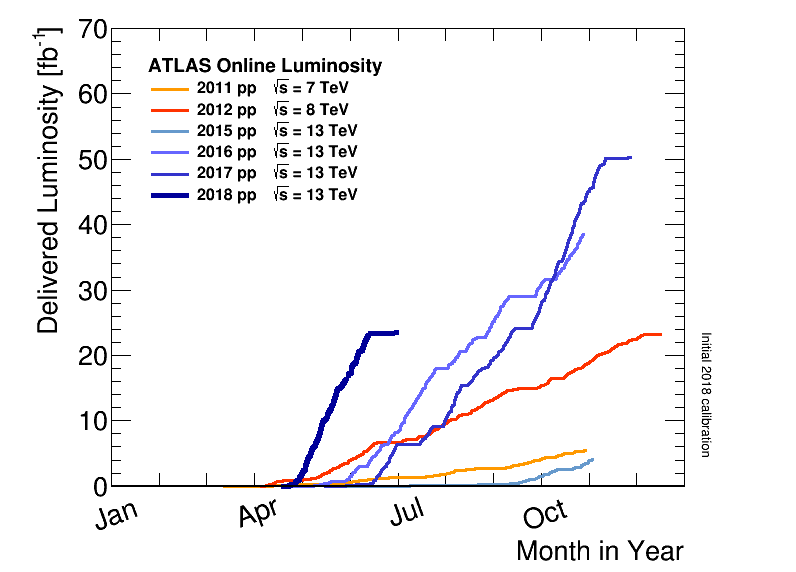
\includegraphics[width=\textwidth]{lhc_lumi_delivered}
\caption{Cumulative luminosity delivered by the LHC over time for each of the years from 2011 to 2018.}
\label{fig:lhc_lumi_delivered}
\end{figure}

\subsection{Layout}\label{subsec:lhc_layout}

The LHC was built inside an already existing tunnel,
which was originally built to house a previous experiment called the Large Electron-Positron Collider (LEP).
The tunnel is roughly circular and $27~km$ in circumference.
It is buried at an average depth of $100~m$ below ground, sloping at a gradient of $1.4\%$ from its deepest point
of $175~m$ to its shallowest at $50m$ below ground.

The ring consists of eight arcs and eight straight regions.
The straight regions are referred to as insertions, and the arcs are called sectors.
The arcs contain dipole magnets which generate the field needed to bend the beams around the ring.
The straight regions are known as insertions.
Four of the insertions are used for particle collisions,
where the two beams are focused with quadrupole magnets in order to collide the greatest number of particles in the smallest possible space.
Each of the four main detector experiments are located at one of these insertions.
The other four insertions are used for beam injection, cleaning, and dumping.
Figure~\ref{fig:lhc_layout} shows a schematic of the layout of the LHC, including locations of the four major detector experiments.

\begin{figure}[h]
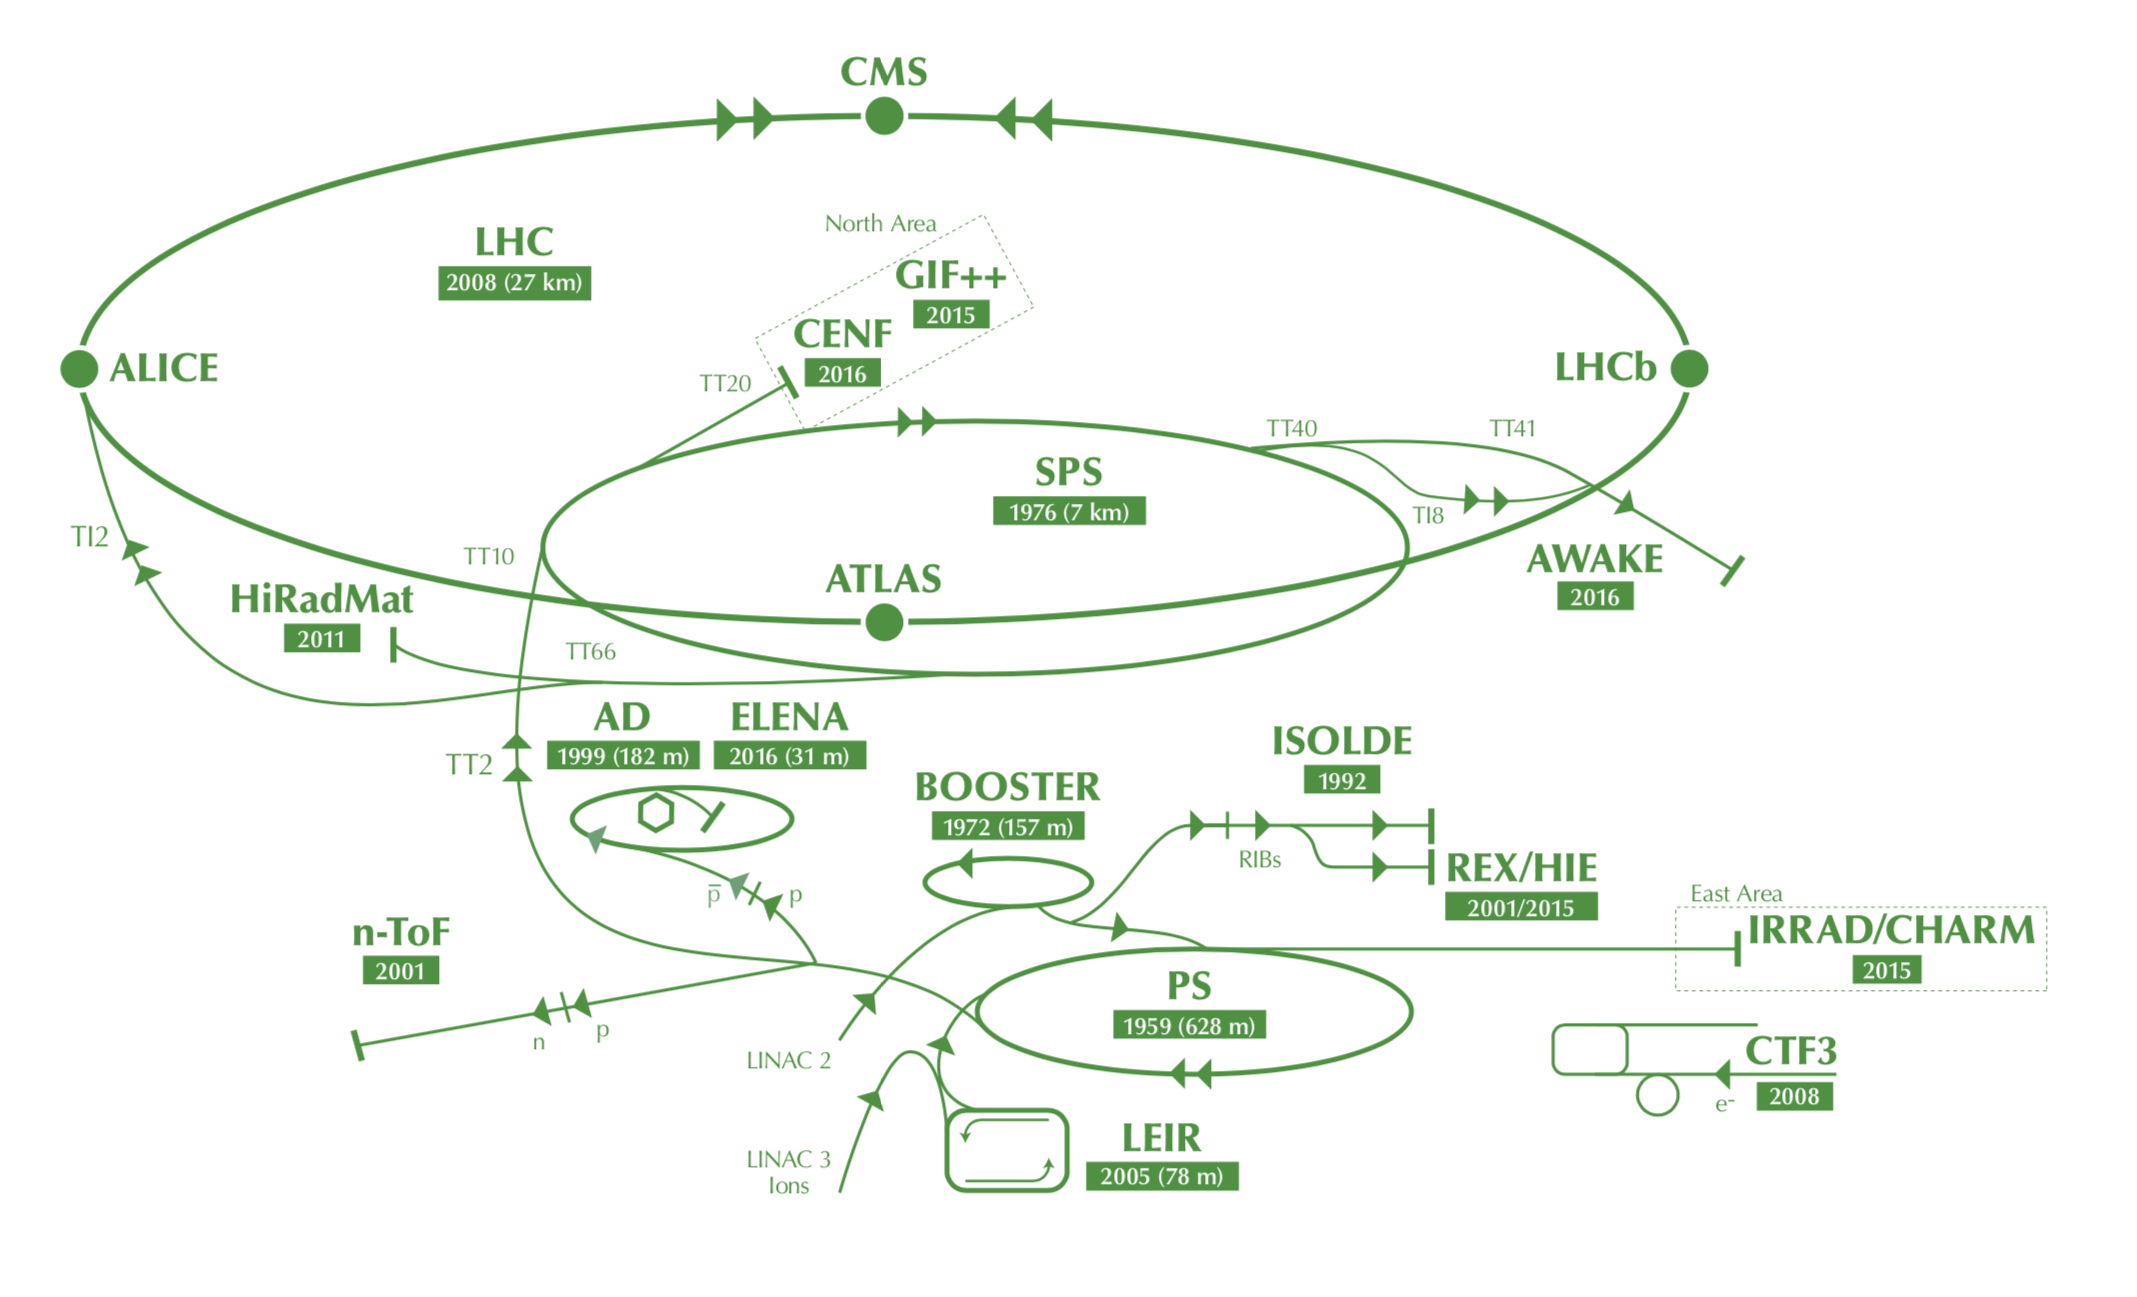
\includegraphics[width=\textwidth]{lhc_layout}
\caption{Schematic of the LHC layout.
The clockwise-rotating beam, shown in red, is referred to as beam 1, and the counter-clockwise-rotating beam, shown in blue, is beam 2.
Locations of the four major detector experiments are labelled.}
\label{fig:lhc_layout}\cite{lhc-machine-2008}
\end{figure}

In figure~\ref{fig:lhc_layout}, the ring is divided into eight octants.
Octants span from the halfway point of one arc to the halfway point of the next arc,
and contain exactly one insertion.

\subsection{Magnets}\label{subsec:lhc_magnets}

\subsubsection{Dipoles}
Each of the eight sectors uses 154 dipole magnets to bend the beams around the ring.
All dipole magnets in a sector are connected in series and cooled in the same continuous crystotat.
Each sector is powered independently.
The magnetic field generated by these magnets points in the y-direction
in order to generate a force that points towards the center of the LHC,
according to the Lorentz force law $\vec{F} = q\left(\vec{E}+\vec{v}\times\vec{B}\right)$.

The maximum beam energy that can be kept in orbit is proportional to the strength of the magnetic field generated by the dipole magnets.
So the design and performance of the dipole magnets is crucial achieving high energies needed by the LHC physics goals.

The dipole magnets are superconducting electromagnets, which generate a field of $8.3~T$.
The superconducting wires are made of $\mathrm{NbTi}$, which has a critical temperature of $10~K$,
but are cooled to and operated at $1.9~K$.
Cooling is done with superfluid helium, which has a very high heat capacity at this temperature.
The wires are made of $7~\mu m$ filaments, thousands of which are twisted together into $15~mm$ strands.
Each cable is then composed of 36 of these strands twisted together.
In order to generate the $8.3~T$ magnetic field, a current of $11.85~kA$ passes through the superconducting wires.

Each dipole magnet is $15~m$ long and weighs $35~t$.
A schematic of the cross-section of an LHC dipole magnet can be seen in figure~\ref{fig:lhc_dipole}.

\begin{figure}[h]
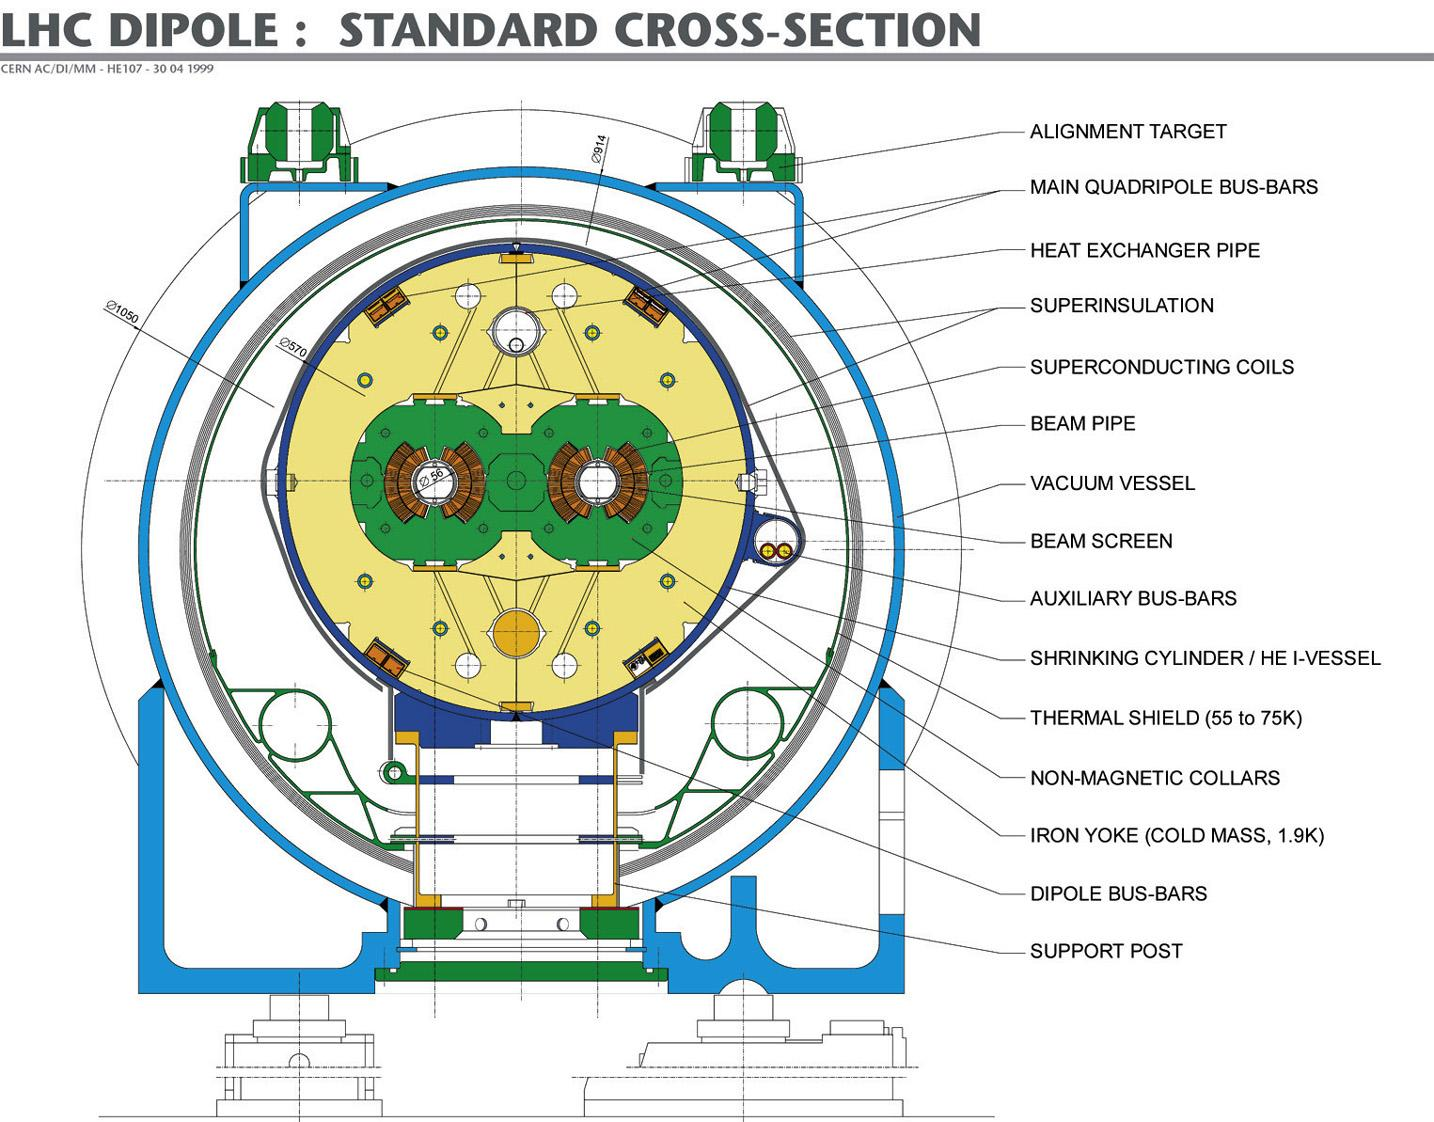
\includegraphics[width=\textwidth]{lhc_dipole}
\caption{Cross-section schematic of an LHC dipole magnet. }
\label{fig:lhc_dipole}\cite{lhc-dipole}
\end{figure}

\subsubsection{Quadrupoles and higher order}

Quadrupole magnets are located near the interaction points of each detector experiment,
for focusing the beams into the smallest possible area before collisions.
When a beam passes through a quadrupole magnet, it is squeezed along one axis perpendicular to the direction of travel of the beam.
It is simultaneously un-squeezed in the direction perpendicular to both the beam and the squeezing direction,
but the magnitude of the un-squeezing is less than the magnitude of squeezing.
When a beam passes through two successive quadrupole magnets with squeezing directions at 90 degrees to each other,
the net effect is a uniform squeezing of the beam towards its center.
Before entering ATLAS, a series of quadrupole magnets squeezes the beams from approximately $0.2~mm$ to less than $20~\mu m$.

Additional higher-order magnets are used in locations around the LHC for beam corrections and damping of oscillations.
There are also special single-bore dipoles which are used to separate the beams in the region of the RF cavities,
so that separate RF cavities can be used for each beam.

\subsection{Radio frequency cavities}\label{subsec:lhc_rf}

Superconducting radio frequency (RF) cavities, operating at $400~MHz$, and $2~MV$, are used to accelerate and store the beams.
The RF cavities accelerate the beams to their nominal energy,
and continue to supply power over the lifetime of the beams to compensate for energy lost through synchrotron radiation.
There are a total of 16 RF cavities, contained within 4 cryomodules.
Figure~\ref{fig:rf_cryo} is a schematic of an RF cavity cryomodule.

\begin{figure}[h]
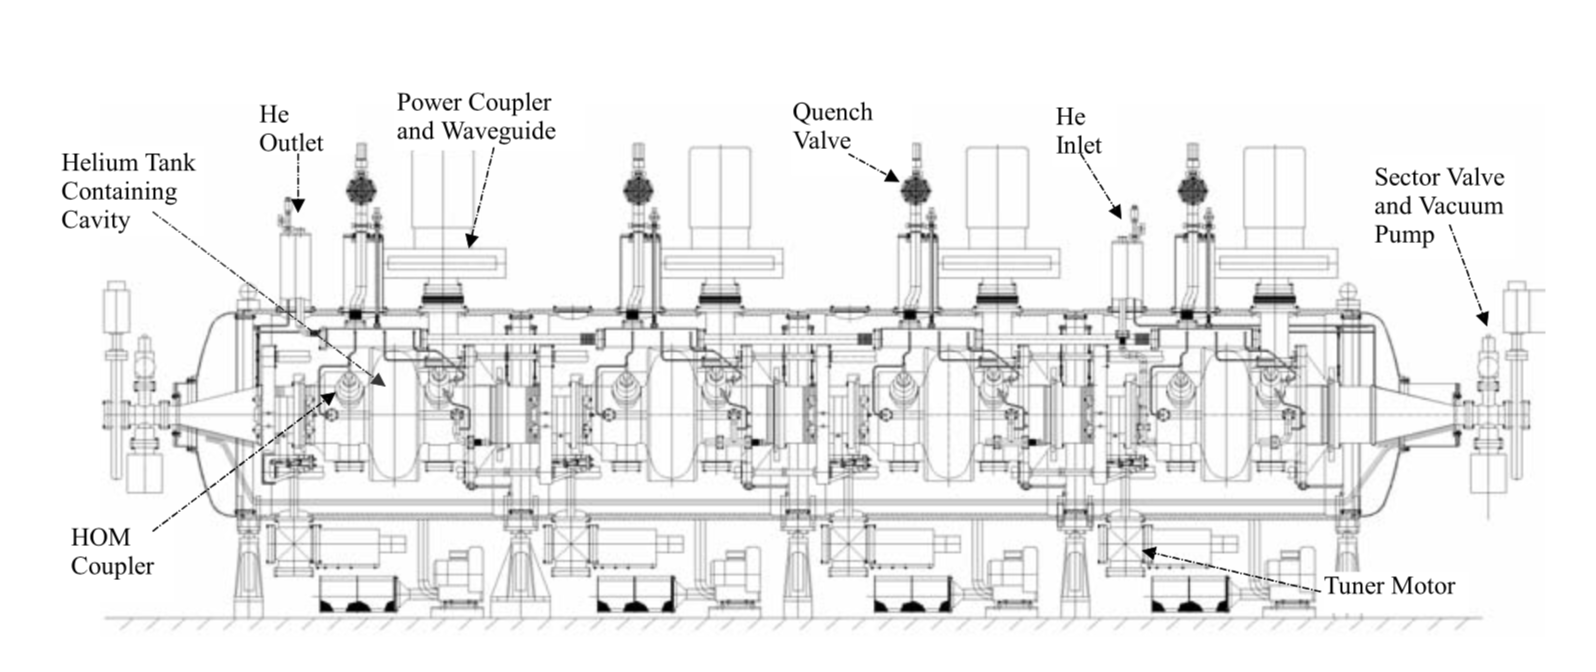
\includegraphics[width=\textwidth]{lhc_rf_cav}
\caption{Schematic of a cryomodule, containing four RF cavities used to accelerate and store the LHC beam.}
\label{fig:rf_cryo}\cite{lhc-machine-2008}
\end{figure}

The RF cavities are tuned such that the resonant frequency of electromagnetic waves inside the cavity is $400~MHz$.
Protons passing through the cavity will be accelerated or decelerated by the electromagnetic field,
depending on their time of arrival in the cavity.
A proton travelling with the exactly the right energy will enter the cavity with just the right timing to experience zero overall force.
Protons travelling slightly too slowly or too quickly will be decelerated or accelerated until their energy is exactly right.
This process results in protons bunching up around the beam, with all protons traveling at the same $13~TeV$ energy.

\subsection{Beams and luminosity}\label{subsec:lhc_beam}

Each beam consists of 2,808 bunches of $10^{11}$ protons each.
The frequency of cycles around the LHC is $11,245~Hz$.
Bunches are mostly evenly spaced, with a few gaps that are needed for beam injection or dumping.
Except for the gaps, bunches are spread out to arrive at the collision points every $25~ns$.
When the gaps are taken into account, actual bunches cross with an average frequency of $30~MHz$.
For a given bunch crossing, an average of 40 proton-proton collisions will occur.
Thus the average number of events delivered to ATLAS per second is approximately 1 billion.\cite{lhc-guide-2017}

Instantaneous luminosity is defined as:
\begin{equation}
\mathcal{L} = \frac{1}{\sigma}\frac{dN}{dt}
\end{equation}

Where $\sigma$ is the physics process under consideration, $N$ is the number of events of that type, and $t$ is time.
Because luminosity is independent of the physics process being considered, it is a characteristic only of the LHC machine.
Luminosity is therefore a useful metric for characterizing the performance of the LHC .

Luminosity is proportional to the square of the number of particles per bunch.
It's also proportional to the number of bunches in each beam, and the frequency of revolution around the accelerator,
according to the equation~\ref{eq:lumi}.

\begin{equation}\label{eq:lumi}
\mathcal{L} = \frac{N_b^2 n_b f_{rev}}{2\pi \Sigma_x \Sigma_y}
\end{equation}
This is why it is most important to maximimize the number of particles per bunch when maximizing luminosity.

In equation~\ref{eq:lumi}, $N_b$ is the number of particles per bunch, $n_b$ is the number of bunches per beam,
$f_{rev}$ is the frequency of revolutions around the LHC, and $\Sigma_x$, $\Sigma_y$ are the transverse widths of the beam in the
x and y direction.

In order to increase luminosity, it is also therefore important to squeeze the beams as much as possible before collisions.
This equation determines how to maximize instantaneous luminosity: put as many protons as possible into as small a space as possible,
and accelerate them as fast as possible.

The peak luminosity delivered to ATLAS by the LHC is $10^{34}cm^{-2}s^{-1}$ for proton-proton collisions,
and $10^{27}cm^{-2}s^{-1}$ for $\mathrm{Pb}$-$\mathrm{Pb}$ collisions.

\section{Coordinates}\label{sec:coordinates}
The coordinate system used in this document is the standard ATLAS coordinate system, detailed here.
For both Cartesian and polar coordinates, the origin is defined as the nominal interaction point.
The z-axis points down the beamline.
The x-y plane is perpendicular to the beamline.
The positive y-direction points up, and the positive x-direction points towards the center of the LHC ring.
The positive z-direction therefore points counterclockwise along the LHC, when viewed from above,
as required by a right-handed coordinate system.

For cylindrical coordinates, the z-axis is defined the same way as for
Cartesian coordinates. The azimuthal angle $\phi$ is the angle
from the positive x-axis, while the polar angle $\theta$ is the angle
from the beamline.

A more convenient measure of angle from the beamline is the
\textit{rapidity}, because rapidity differences are invariant under Lorentz boosts in the
z-direction.
Rapidity is defined as:
\begin{equation}
y = \frac{1}{2}\ln\frac{E+p_z}{E-p_z}
\end{equation}

Another frequently used quantity is the
\textit{pseudorapidity}, which is defined as:
\begin{equation}
\eta = -\ln\frac{\theta}{2}
\end{equation}

Pseudorapidity differences are also invariant with respect to
longitudinal Lorentz boosts. In the limit where $p_T \ll m$, rapidity and
pseudorapidity are equal.

Pseudorapidity ranges from zero to plus or minus infinity.
The x-y plane, which is perpendicular to the beamline, is described by a pseudorapidity $\eta=0$.
The z-axis, which is parallel to the beamline, is described by pseudorapidity $\eta=\pm\infty$

Finally, a distance measure in $\eta-\phi$ space is often used, especially when describing jets.
This distance, $\Delta R$ is defined as:

\begin{equation}
\Delta R = \sqrt{\Delta\eta^2+\Delta\phi^2}
\end{equation}

\section{Magnet Systems}\label{sec:magnet_systems}
The two ATLAS magnet systems are used to curve the tracks of charged particles passing through the detector,
so that their momenta can be measured.

The layout of the magnet systems can be seen in figure~\ref{fig:magnet_layout}.

\begin{figure}[!htbp]
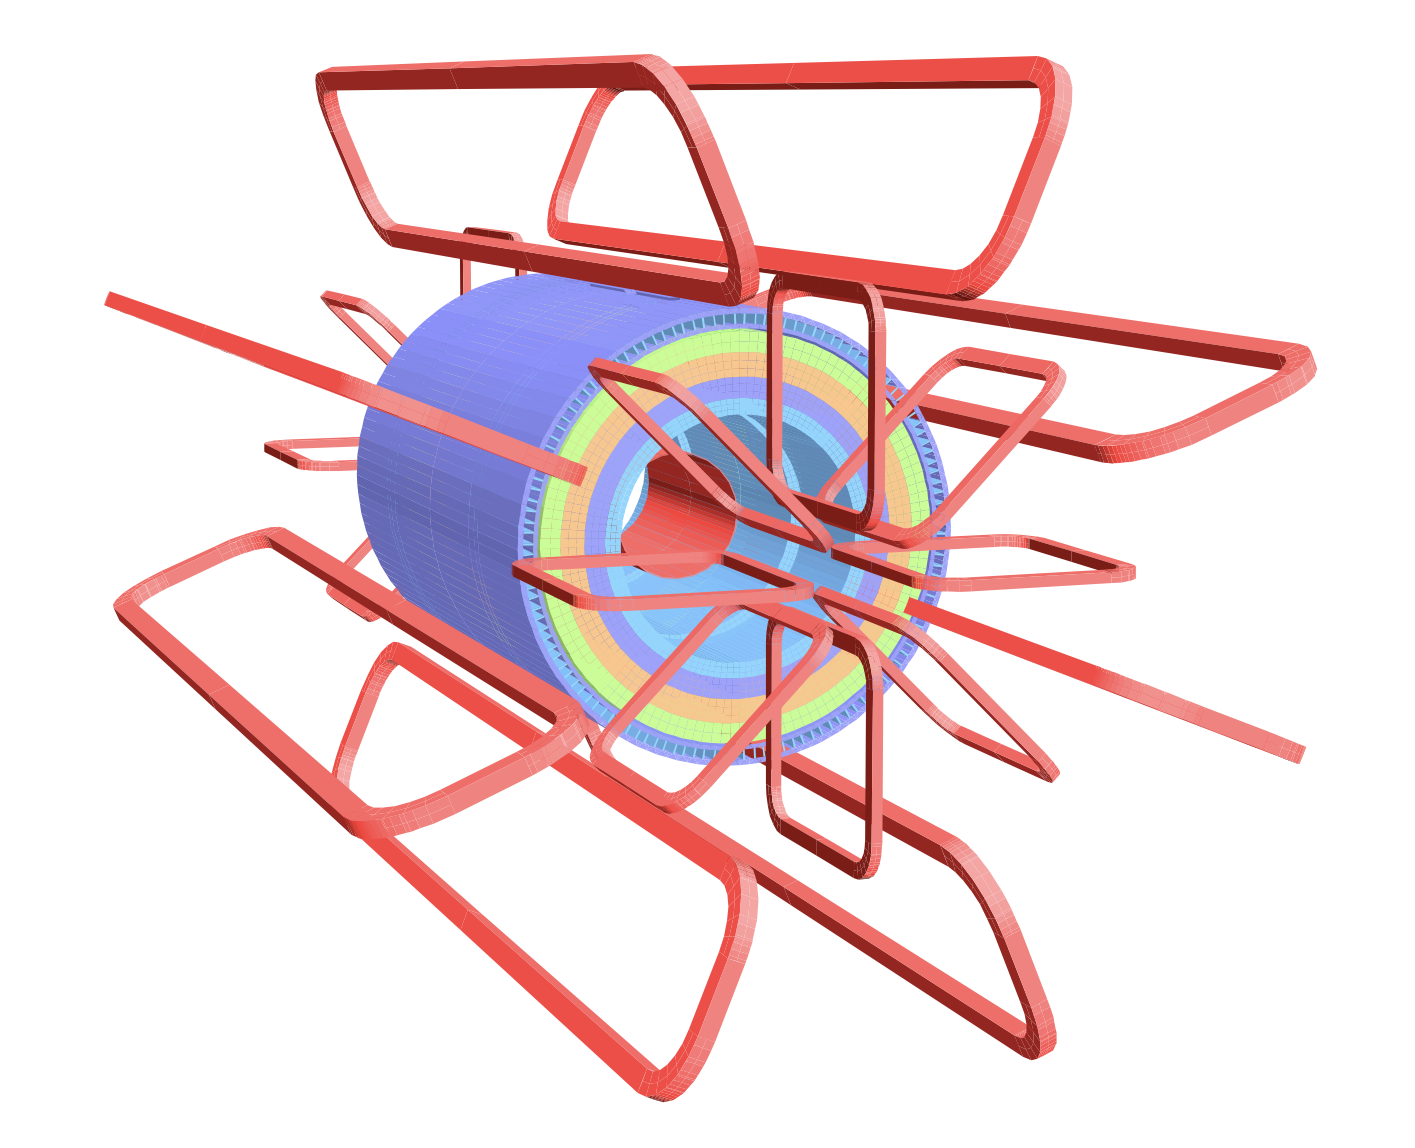
\includegraphics[width=\textwidth]{magnet_layout}
\caption{A diagram showing the layout of the ATLAS magnet system.
The central solenoid is used to apply a force that curves the trajectories of charged particles in the inner detector.
In red are the toroid coils, used to bend the tracks of charged particles passing through the muon spectrometer.}
\label{fig:magnet_layout}
\end{figure}

The first magnetic field is produced by the central solenoid, which surrounds the entire inner detector,
and is surrounded by the barrel calorimeters.
It generates a uniform $2~T$ axial magnetic field in the inner detector.
The coils are made of Al-stabilized NbTi. The length is $5.8~m$, and the outer diameter is $2.56~m$\cite{atlas-detector-2008}.

The second magnet system, used to bend the trajectories of muons passing through the muon spectrometer,
has a more complicated geometry.
It consists of a barrel toroid section, and two symmetrical end-cap toroids.
The exact shape of the resulting magnetic field is quite complex,
but roughly runs in a circular direction around the calorimeters.

The axial length of the barrel toroid is $25.3~m$, and the outer diameter measures $20.1~m$.
The average field strength is $0.5~T$ and the superconducting material used is similar to that used in the
central solenoid\cite{atlas-detector-2008}.
The magnetic field in the region $|\eta|<1.4$ is dominated by the barrel toroid,
while the end-cap field dominates the region $1.6 < |\eta| < 2.7$.
The region $1.4 < |\eta| < 1.6$ is the transition region, where both sources contribute significantly to the magnetic field.

Figure~\ref{fig:toroid_end_view} shows an end-on view of the barrel toroid, after installation,
and before the calorimeters are inserted.

\begin{figure}[h]
\includegraphics[width=\textwidth]{toroid_end_view}
\caption{A picture of the ATLAS barrel toroid after installation. In
  the center of the image is the calorimeter and central solenoid,
  before being moved into the final position.}
\label{fig:toroid_end_view}
\end{figure}

The end-cap toroids are used to generate the magnetic field for muons passing through the end-cap region of the muon spectrometer.
The properties and geometry of the end-cap toroids are similar to the barrel toroid,
with peak magnetic field reaching $4.1~T$\cite{atlas-detector-2008}.

\section{Inner Detector}\label{sec:inner_detector}
The inner detector consists of silicon pixel detectors, silicon strip detectors, and transition radiation trackers.
It covers a region from $R = 33~mm$ to $R = 1082~mm$ and $|\eta| = 0$ to $|\eta| = 2.5$.
The entire inner detector is immersed in a $2~T$ magnetic field, generated by a
solenoid coil which surrounds it.\cite{atlas-detector-2008}
The layout of inner detector subsystems is shown in figure~\ref{fig:inner_detector_quarter}.

\begin{figure}[h]
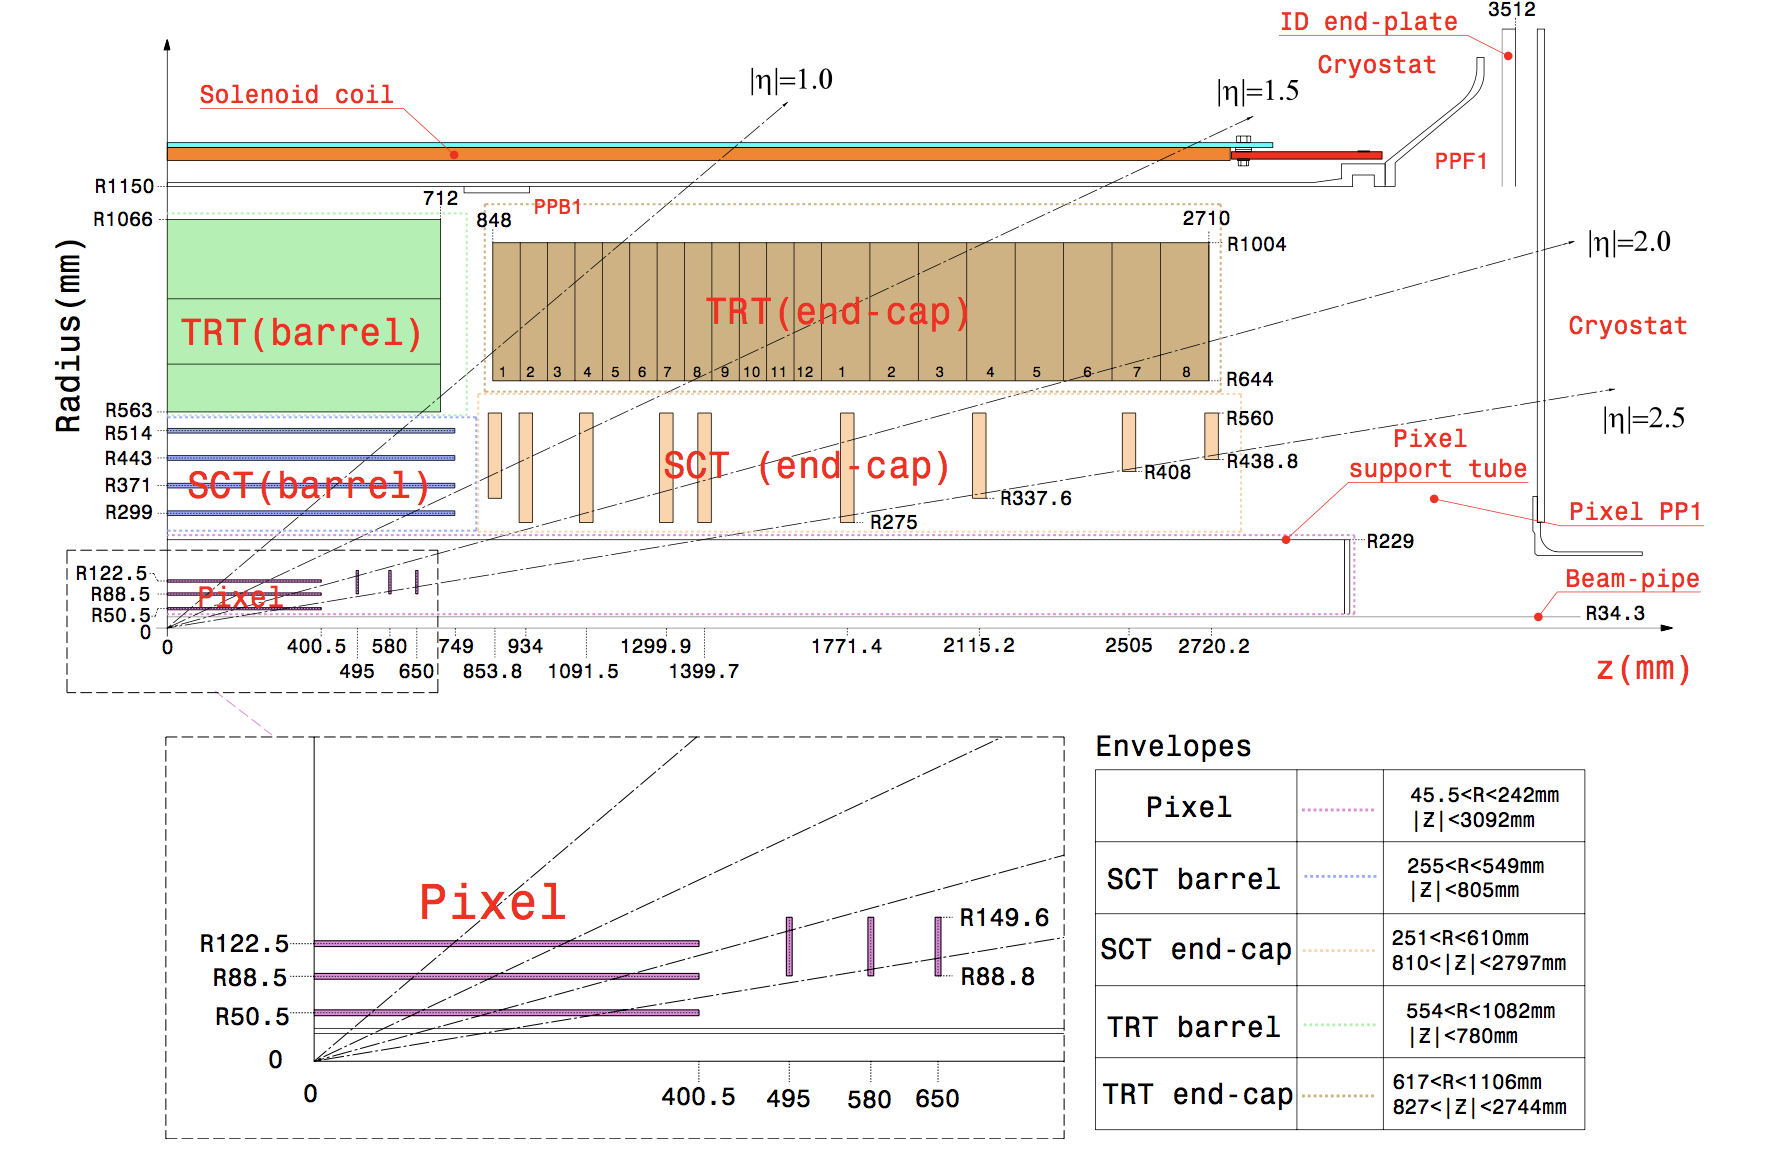
\includegraphics[width=\textwidth]{inner_detector_quarter}
\caption{A quarter-section plan showing the layout of inner detector susbystems and their dimensions.
Not shown is the innermost layer of the pixel detector, the IBL, which was installed in May 2014.}
\label{fig:inner_detector_quarter}
\end{figure}

\subsection{Pixel Detector}\label{subsec:pixel}

The innermost layer of ATLAS detectors is the pixel system.
Since it lies closest to the interaction point, the pixel system experiences the highest flux of any ATLAS subdetector.
This means that the pixel detector must have the greatest radiation hardness, greatest resolution,
and greatest occupancy of any subdetector.\cite{atlas-detector-2008}
The pixel system consists of 1744 solid-state pixel sensors, arranged into a barrel region and two endcap regions.
In total, there are 80.4 million pixel readout channels.\cite{atlas-detector-2008}

\subsubsection{Layout}
The barrel region consists of four concentric cylindrical layers, coaxial with the beamline.
The two endcap regions are each made up of three disks, arranged perpendicular to the beamline.

The pixel barrel envelope covers a region from $z = 0$ to $|z|  = 400.5~mm$.
The four layers are located at increasing distances from the beamline, at $R = 33~mm, 50.5~mm, 88.5~mm, 122.5~mm$.

The six endcap disks are located at $|z| = 495~mm, 580~mm, 650~mm$ and cover the region $88.8~mm < R < 149.6~mm$.\cite{atlas-detector-2008}

Figure~\ref{fig:inner_detector_quarter} shows a quarter-section of
the entire inner detector, as well as a detailed view of the pixel
subsystem, not including the Insertable B Layer (IBL), which was
installed in 2014.

\subsubsection{Sensors}
The ATLAS pixel sensors are solid-state silicon detectors.
The basic operating principle of a solid-state detector is that charged particles passing through the material
generate electron-hole pairs, which are accelerated towards opposite ends of the material via an electric field.
This generates a current, which can be measured by charge-sensitive sensors at the edge of the material.\cite{spieler-2005}

In a silicon detector, the active material is a pn junction, operated with a reverse bias voltage,
until fully depleted.
This reduces the thermal noise from free charge carriers to a low enough level that electron-hole pairs
from signal particles can be detected.\cite{spieler-2005}

In ATLAS, the pixel sensors consist of an n-type bulk, with $p^+$ implants on the back side and $n^+$ implants on the front side.
Before irradiation, the active pn junction region exists between the n-type bulk and $p^+$- implanted side.
Irradiation leads to the reduction in the effective doping concentration,
until the bulk material undergoes type inversion.
After type inversion, the active pn junction region switches to the $n^+$-doped side.\cite{pixels-2008}
This process is illustrated in figure~\ref{fig:pixel_type_inversion}.

This $n^+$-in-$n$ design allows the sensors to continue to operate both before and after large doses of radiation.

Each pixel tile has 47232 pixels, laid out in a grid of 144 columns by 328 rows.
Some of the pixels are grouped to common read-out channels, resulting in 46080 read-out channels.
This grouping is done so that an equal number of read-out channels can be connected to each of
the 16 front-end read-out chips.\cite{pixels-2008}

In 128 of the columns, each pixel implant is $382.5\times30~\mu m^2$, with pitch (center-to-center distance) of  $400\times50~\mu m^2$.
In the remaining 16 columns, the pixel sizes are $582.5\times30~\mu m^2$, with a pitch of  $600\times50~\mu m^2$.\cite{pixels-2008}

\begin{figure}[h]
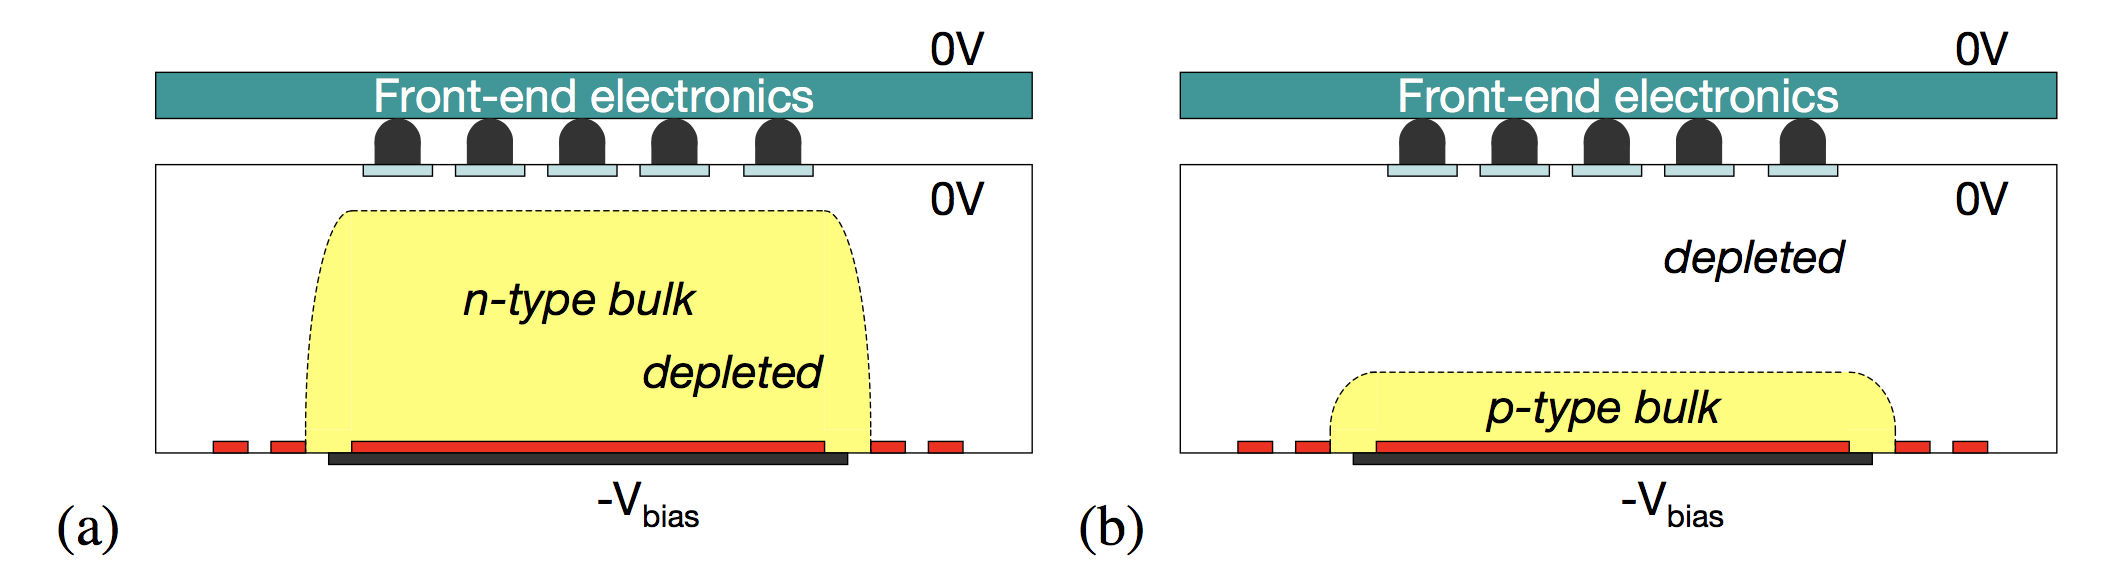
\includegraphics[width=\textwidth]{pixel_type_inversion}
\caption{Graphic illustrating how $n^+$-in-$n$ pixel sensors continue to operate after the type inversion that results from irradiation.
In (a), the unirradiated state, the bulk is n-type, and the depletion zone occurs between the $p^+$-doped back side.
After type inversion, in (b), the depletion zone occurs between the now p-type bulk and the $n^+$-doped front side.
\cite{pixels-2008}}
\label{fig:pixel_type_inversion}
\end{figure}

\subsubsection{The IBL}
A major upgrade that occurred during the long shutdown in 2014 was to install the Insertable B-Layer (IBL) to the pixel detector.
The IBL became the fourth and innermost layer of the pixel detector.
The IBL provides several key improvements to the tracking system, which will allow the pixel detector to maintain
good performance even in the higher-luminosity environment that will be present in the High Luminosity LHC (HL-LHC).\cite{ibl-tdr}
The IBL does this by improving tracking robustness against module failures,
adding measurement redundancy to mitigate the effects of pileup,
and adding an additional measurement closer to the interaction point.\cite{ibl-tdr}

As part of the IBL insertion project, the original beam pipe was removed, and replaced with a smaller-radius beampipe.
Precision tooling and methods for insertion were developed and practiced for two years before the procedure was finally carried out.
The tolerances were extremely tight, with only a $0.2~mm$ gap between the IBL and inner supporting tube.\cite{ibl-website}.
An image of the IBL being inserted can be seen in figure~\ref{fig:ibl_insertion}

\begin{figure}[h]
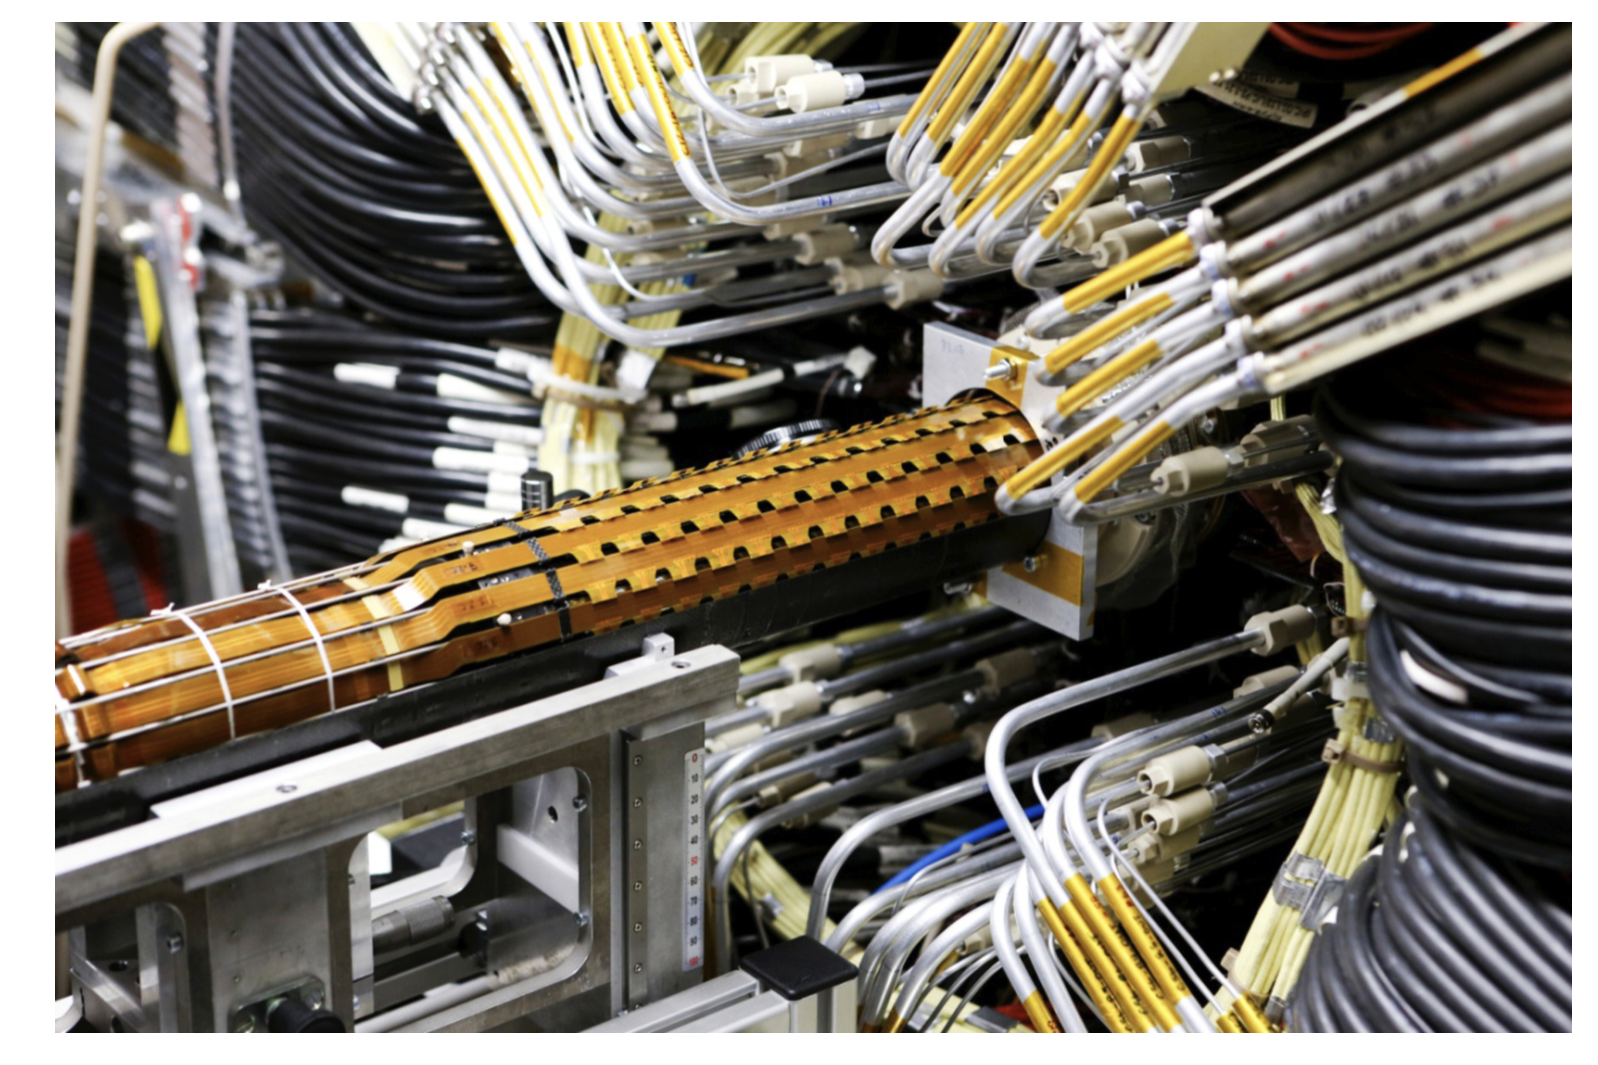
\includegraphics[width=\textwidth]{ibl_insertion}
\caption{The IBL as it was inserted into the pixel detector}
\label{fig:ibl_insertion}\cite{ibl-website}
\end{figure}

\subsection{Silcon Strip Tracker}\label{subsec:sct}

After the pixel detector system, the next innermost subdetector is the SemiConductor Tracker, or SCT .
The SCT consists of 4088 modules, with a total silicon surface area of $63~m^2$.\cite{atlas-detector-2008}
The SCT sensors are silicon strips rather than pixels.
In order to obtain two-dimensional resolution, SCT modules are paired back-to-back at a small stereo angle.

\subsubsection{Layout}
Like the pixel system, the SCT barrel region consists of four concentric cylindrical layers, coaxial with the beamline.
The two endcap regions are each made up of nine disks, arranged perpendicular to the beamline.

The SCT barrel envelope covers a region from $z = 0$ to $|z|  = 746~mm$,
and the four layers are located at increasing distances from the beamline,
at $R = 299~mm, 371~mm, 443~mm, 514~mm$.\cite{sct-barrel-2006}

The nine endcap disks on each side range from $|z| = ~mm$ to $|z| = ~mm$,
and cover the region $275~mm < R < 560~mm$.\cite{atlas-detector-2008}

The modules are arranged in back-to-back pairs at a stereo angle of $40~mrad$, in order to provide two-dimensional resolution.

\subsubsection{Modules}
Like in the pixel system, the SCT sensors are solid-state silicon detectors.
Instead of pixels, the base unit is a strip of silicon, ranging in length from $6$ to $13~cm$.
These strips are made of p-type silicon, and are embedded in n-type silicon. The average pitch is $80~\mu m$.\cite{sct-2010}

The resolution resulting from this design is $17~\mu m$ in the $r-\phi$ direction, and $580~\mu m$ in the z-direction.\cite{sct-2010}

\subsection{Transition Radiation Tracker}\label{subsec:trt}
Moving outwards from the pixel system and SCT, the final inner detector subsystem is the transition radiation tracker, or TRT .
Unlike the pixel or SCT systems, the TRT uses proportional drift tubes, referred to as straws, as sensors.

To make accurate track measurements, the TRT relies on a larger number of hits over a longer distance than the pixel system or SCT .
Since the TRT measures approximately 36 hits per track, and makes measurements over a longer distance,
less spatial precision is required per hit.\cite{atlas-detector-2008}

The TRT only provides tracking information in the $R-\phi$ direction, unlike the pixel and SCT systems,
which each provide three-dimensional tracking information.

The main purpose of the TRT is to provide additional tracking information.
But transition radiation photons generated in the TRT gas-filled tubes can also aid in electron identification.\cite{atlas-detector-2008}

\subsubsection{Operating Principle}
The TRT uses proportional drift tubes to detect charged particles.
A tube is filled with a mixture of two or more gases, including an inert gas such as Xenon.
And an electric field is applied across the tube.
When a charged particle passes through the tube, ion pairs are generated from the inert gas.
Positive and negative ions drift in opposite directions, towards the cathode and anode, respectively.
If a particle's energy is completely absorbed in the tube, the number of ions produced in stopping the particle is
proportional to the original energy of the particle.\cite{knoll-2000}

In addition to the inert gas, it is common to add another gas, such as Carbon Dioxide, to stabilize the ionization process.
This additional gas is referred to as a quencher gas.

\subsubsection{Layout}

Like the pixel system and SCT systems, the TRT consists of a barrel region and two end-cap regions.
In the barrel region, straw tubes are arranged coaxial to the beamline and measure $144~cm$ in length.
In the end-cap region, straw tubes are arranged radially, and measure $37~cm$ in length.\cite{atlas-detector-2008}

The TRT barrel envelope covers a region from $z = 0$ to $|z|  = 780~mm$, and $554 < R 1082~mm$,
and the end-cap envelop covers a region from $z = 848$ to $|z|  = 2710~mm$, and $644 < R 1004~mm$.
This provides tracking coverage out to $|\eta| = 2.0$.\cite{atlas-detector-2008}

A charged track passing trough the TRT will typically produce 36 hits.
Each straw provides a hit resolution of $130~\mu m$.
There are 351,000 total readout channels.

\begin{figure}[h]
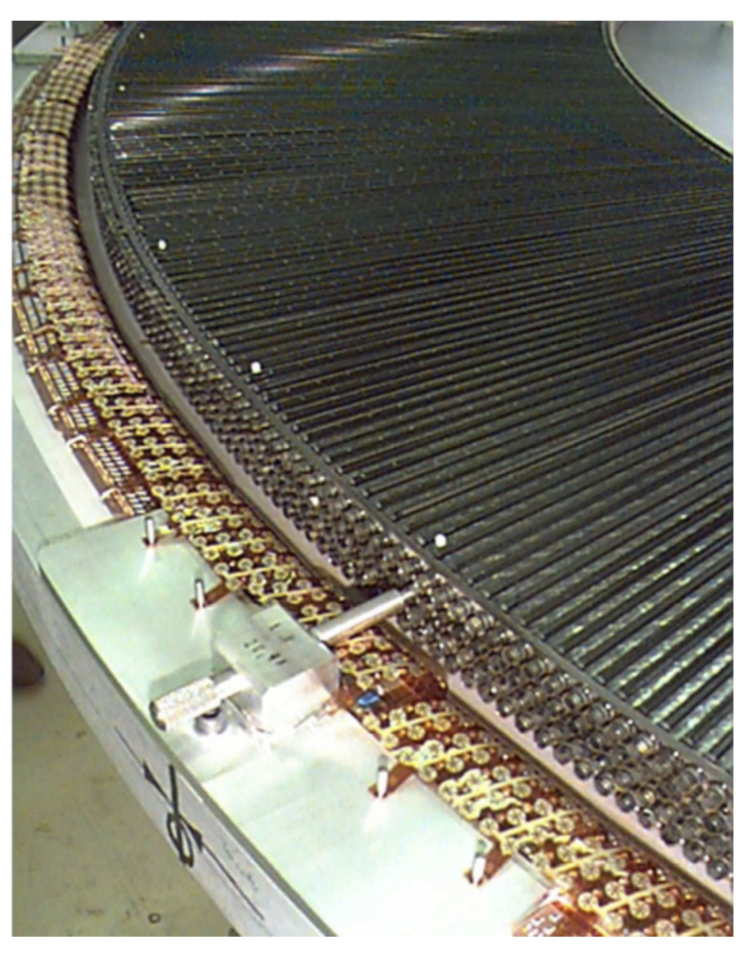
\includegraphics[width=\textwidth]{trt_end_cap}
\caption{Part of a TRT end-cap, showing the radial layout of the $37~cm$ straw tubes.}
\label{fig:trt_end_cap}\cite{trt-2013}
\end{figure}

\subsubsection{Sensors}

The TRT straw tube walls are constructed of two layers of $25~\mu m$-thick Kapton film.
The Kapton is coated with a $0.2~\mu m$-thich layer of aluminum, followed by a $6~\mu m$-thich layer of carbon-polyimide.
The Aluminum layer serves to provide electrical conductivity, and the carbon-polyimide layer is to protect the aluminum.
The two Kapton layers are sealed together with a $5~\mu m$-thick polyurethane layer.\cite{trt-2013}
The TRT straw wall design is shown in figure~\ref{fig:trt_straw_wall}

\begin{figure}[h]
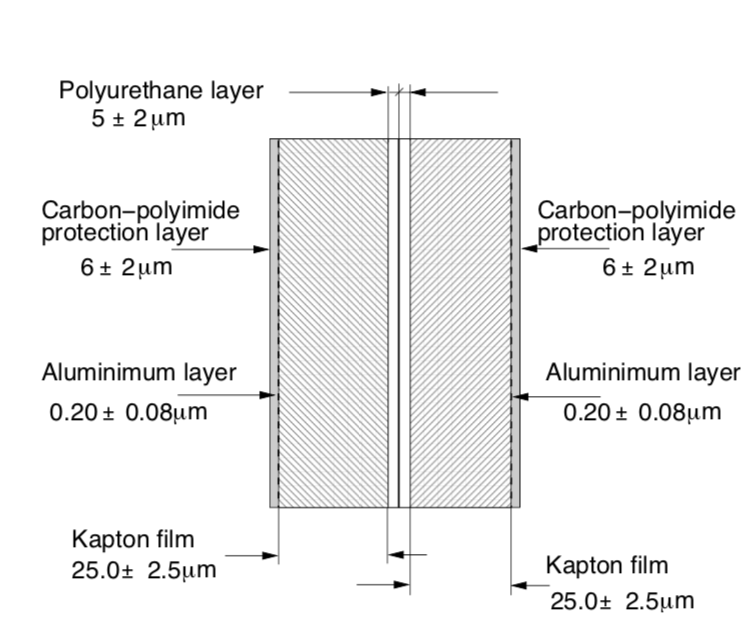
\includegraphics[width=\textwidth]{trt_straw_wall}
\caption{Schematic of the TRT straw wall design. Two coated Kapton layers are sealed together with polyurethane.}
\label{fig:trt_straw_wall}\cite{trt-2013}
\end{figure}

The straws are filled with a mixture of $70\%~\mathrm{Xe}$, $27\%~\mathrm{CO_2}$,
and $3\%~\mathrm{O_2}$.
Carbon dioxide is used as a quencher gas, which is needed to guarantee that the ionization procedure is stable.
The addition of a small amount of oxygen increases the voltage difference between the working point and the breakdown voltage,
further stabilizing the process.\cite{trt-2013}

In order to maximize hit efficiency, the straw diameter should be as large as possible.
But there is a tradeoff: as straw diameter increases, so does the drift time.
The optimal diameter to ensure acceptable time resolution for $25~ns$ bunch-spacing was chosen as $4~cm$.\cite{trt-2013}

\section{Calorimeters}\label{sec:calorimeters}

The ATLAS calorimeters are designed to absorb and measure the energy of both electromagnetic and hadronic showers.
Different materials and geometries are used for different calorimeter subsystems, but the operating principle is the same.
In each calorimeter, there is an absorber medium, and a sampling medium.
When a particle strikes the absorber medium, it triggers a shower of particles which then pass into the sampling medium.
The sampling medium is ionized by these showering particles, and instrumentation is used to measure the amount of ionization.
In order to accurately measure shower energy, the ATLAS calorimeters are designed to fully absorb both electromagnetic and hadronic showers.

The innermost calorimeter is a high-granularity detector optimized for measuring electromagnetic showers.
Lead is used as an absorber and LAr as the sampling medium.
It covers the range $|\eta| < 3.2$.

The outer calorimeter has a coarser granularity and is optimized for measuring jets and $E_{T miss}$ .
It consists of scintillator tiles and uses steel as the absorber.

In addition to the EM and hadronic calorimeters, there is copper-tungsten/LAr calorimeter providing coverage out to
$|\eta| < 4.9$.
This is known as the forward calorimeter, or FCal.

The layout of the ATLAS calorimeter system can be seen in figure~\ref{fig:calo_full}

\begin{figure}[h]
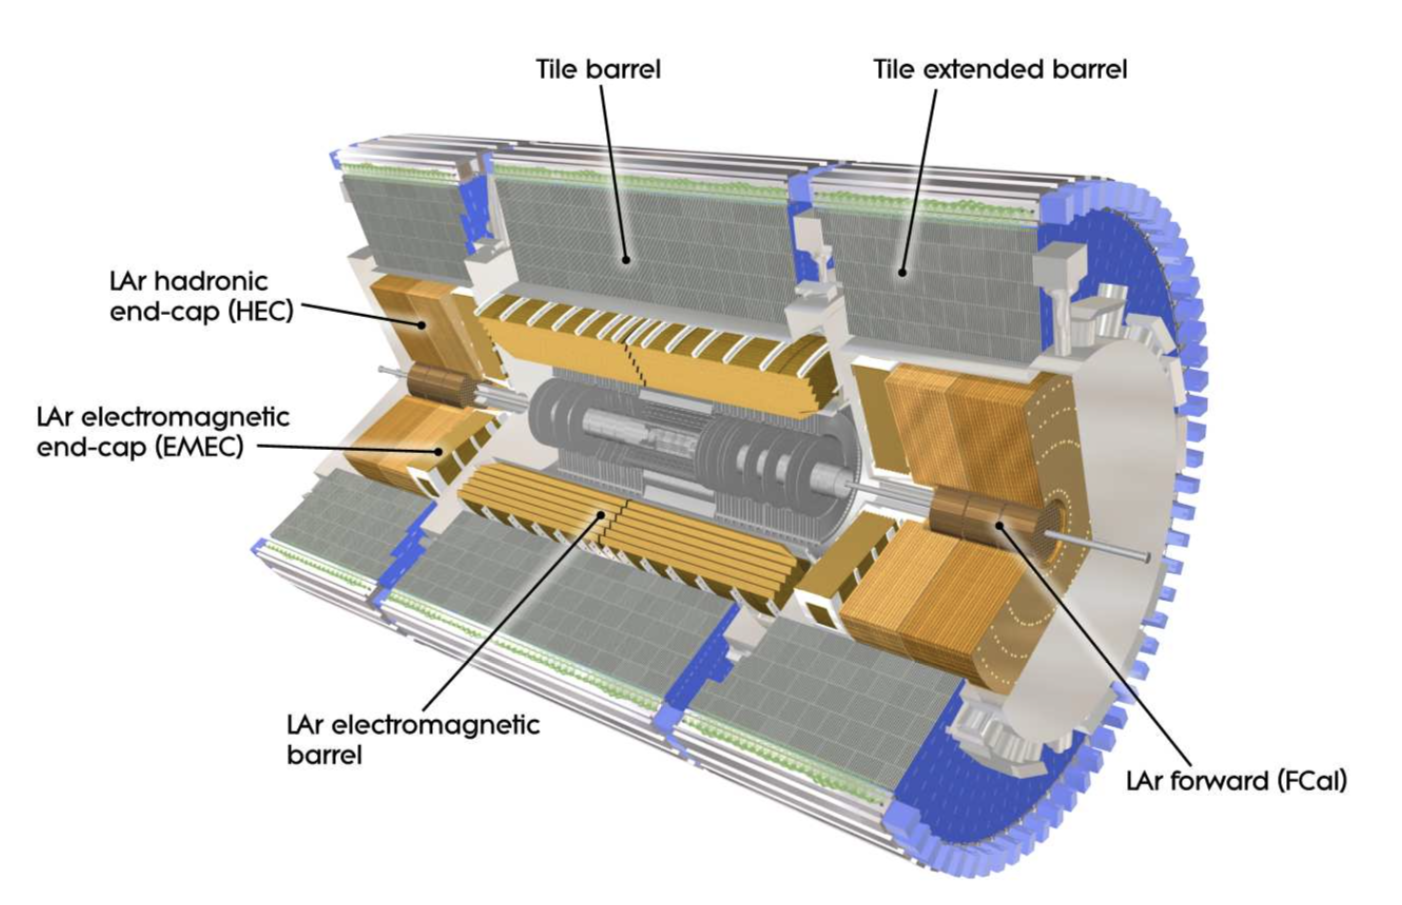
\includegraphics[width=\textwidth]{calo_full}
\caption{Layout of the ATLAS calorimeter system.}
\label{fig:calo_full}\cite{atlas-detector-2008}
\end{figure}

\subsection{Electromagnetic Calorimeters}\label{subsec:em_cal}

The electromagnetic calorimeter is located just outside the solenoid that surrounds the inner detector.
It is optimized for measuring the energy of electromagnetic showers.
The EM calorimeter is also designed to measure the direction of neutral particles, which cannot be tracked by the inner detector.

In the barrel region, the EM calorimeter covers the range $|\eta| < 1.475$.
In the end-cap region, it covers a range of $1.375 < |eta| < 3.2$.

The calorimeters have to be thick enough to fully absorb shower energy and to minimize punch-through into the muon system.
The EM calorimeter depth was designed to be 22 interaction lengths $\left(X_0\right)$ in the barrel, and $24~X_0$ in the end-caps.
An interaction length is defined as the average distance traveled by a particle through a material when it has lost
$1 - 1/\mathrm{e}$ of its original energy.\cite{em-calo}

The calorimeters consist of accordion-shaped lead absorber plates with copper-kapton electrodes in between.
The accordion shape provides full symmetry in $|\phi|$ with no gaps.
The absorber plates are grounded and the electrodes are kept at $2000~V$ in the barrel region and between
$1000$ and $2500~V$ in the end-cap region.
The whole system is immersed in liquid argon.\cite{atlas-detector-2008}

A particle passing through the lead absorbers generates a shower of particles, which ionize the LAr.
Due to the electric field between the absorber plates and electrodes, ions drift towards the electrodes.
This generates a pulse in the electrodes which can then be recorded.

The calorimeter cells are arranged into three layers, with highest granularity closest to the interaction point.
Cells in layer 1 have a granularity of $\delta\phi \times \delta\eta = 0.0245 \times 0.0031$.
This very fine segmentation is useful in accurately determining the direction of incoming particles.
It is also useful in discriminating between an individual photons and a neutral $\pi$ meson decaying to two photons.\cite{em-calo}

In the second layer, the granularity is reduced $\delta\phi \times \delta\eta = 0.0245 \times 0.025$.

In the third and final layer, the granularity is further reduced to $\delta\phi \times \delta\eta = 0.0245 \times 0.05$.

The geometry of the EM calorimeter cells can be seen in figure~\ref{fig:em_calo}

Inside the innermost layer of the barrel EM calorimeter is an $11~mm$-thin presampler, covering a range of $|\eta| < 1.8$.
The purpose of this presampler is to correct for energy lost to material upstream of the EM calorimeter.

\begin{figure}[h]
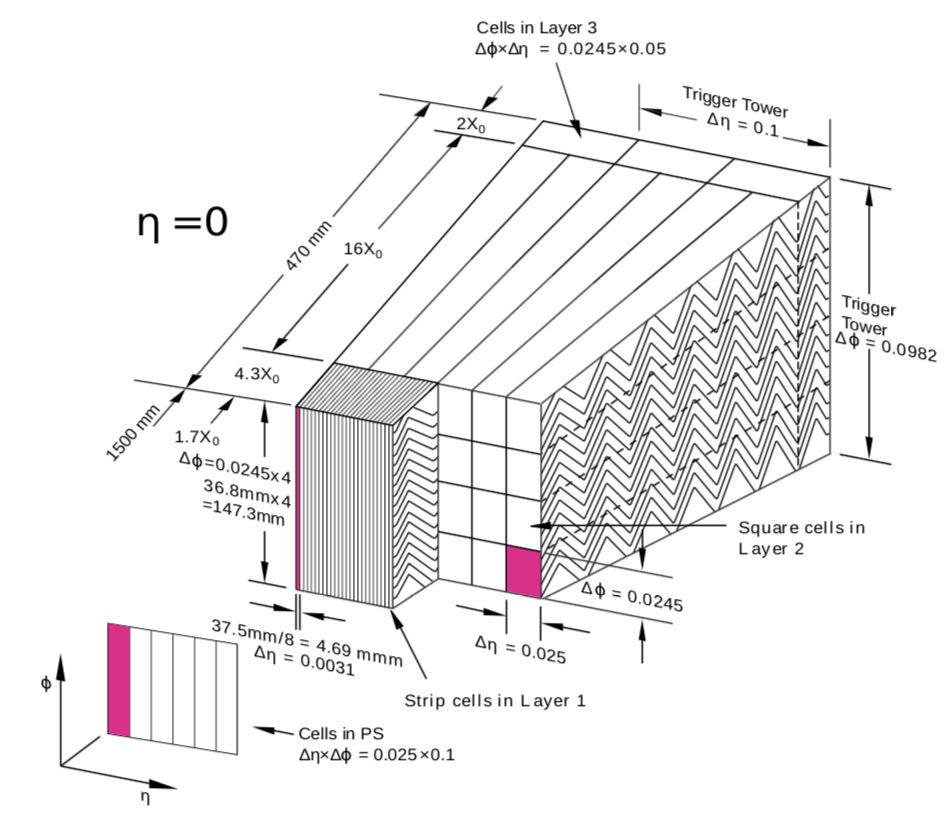
\includegraphics[width=\textwidth]{em_calo}
\caption{Schematic of EM calorimeter, showing the granularity of each layer.}
\label{fig:em_calo}\cite{em-calo}
\end{figure}

\subsection{Hadronic Calorimeters}\label{subsec:had_cal}

The most important ATLAS subdetector for measuring jets is the hadronic calorimeter system.

The hadronic calorimeter system consists of central and extended tile calorimeter barrels, two end cap calorimeters,
and a forward calorimeter.

\subsubsection{Tile calorimeters}

The central tile barrel covers the range $|\eta|<1.0$, the extended tile barrels cover the range $0.8 < |\eta| < 1.7$,
and the end-cap calorimeters cover the range $1.5 < |\eta| < 3.2$.
The forward calorimeters (FCal) cover the extreme forward region, $3.1 < |\eta| < 4.9$.

The central barrel is $5.8~m$ long, and the extended barrels are each $2.6~m$ long.
Both the central and extended barrels cover the range $2.28~m < R < 4.25~m$.
Each of the three tile calorimeters is composed of 64 wedge-shaped modules.
The geometry of the hadronic calorimeter system, not including the end-caps, can be seen in figure~\ref{fig:calo_full}.

The hadronic calorimeters in the central and extended barrel regions are tile calorimeters.
They consist of alternating steel absorber plates and scintillating tiles.
Particles that pass through the steel plates generate hadronic showers.
The hadrons from these showers then stimulate the production of photons in the scintillating tiles.
Those photons are then collected by photomultiplier tubes, producing a current that can be measured.
A wavelength-shifting fiber is used to convert the ultraviolet photons produced in the scintillator into optical photons
before entering the photomultipliers.

A schematic of a tile calorimeter module can be seen in figure~\ref{fig:tile_cal_module}

\begin{figure}[h]
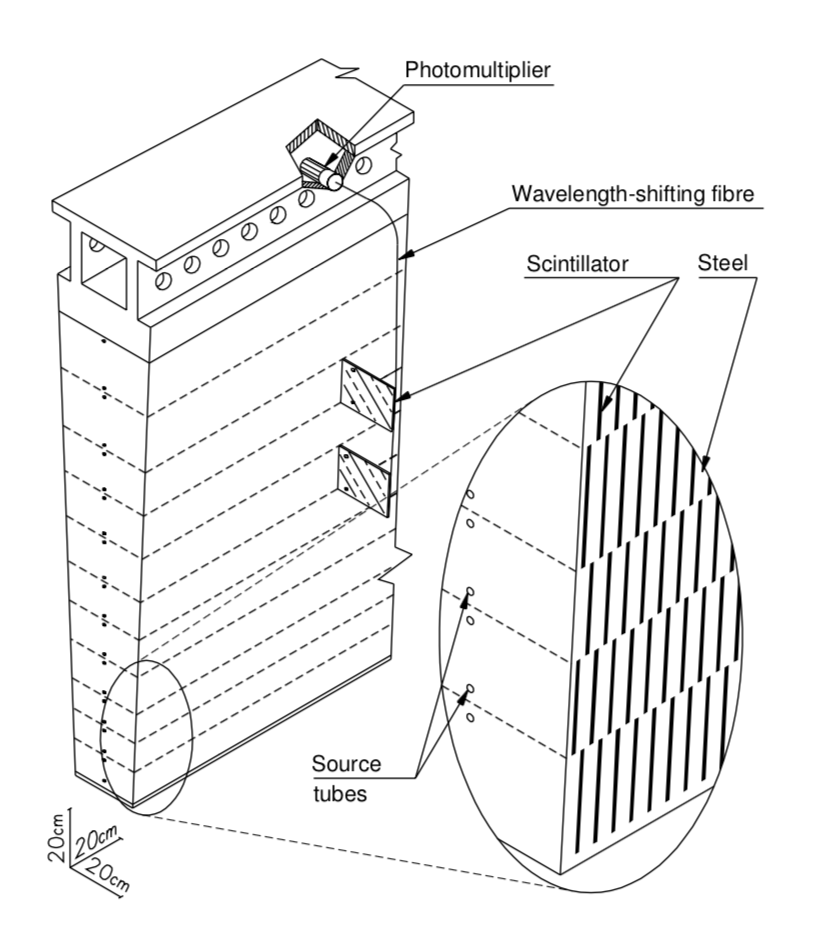
\includegraphics[width=\textwidth]{tile_cal_module}
\caption{Schematic of EM calorimeter, showing the granularity of each layer.}
\label{fig:tile_cal_module}\cite{atlas-detector-2008}
\end{figure}

The $\eta$- and depth-dependent segmentation of the tile calorimeter modules can be seen in figure~\ref{fig:tile_cal_granularity}

\begin{figure}[h]
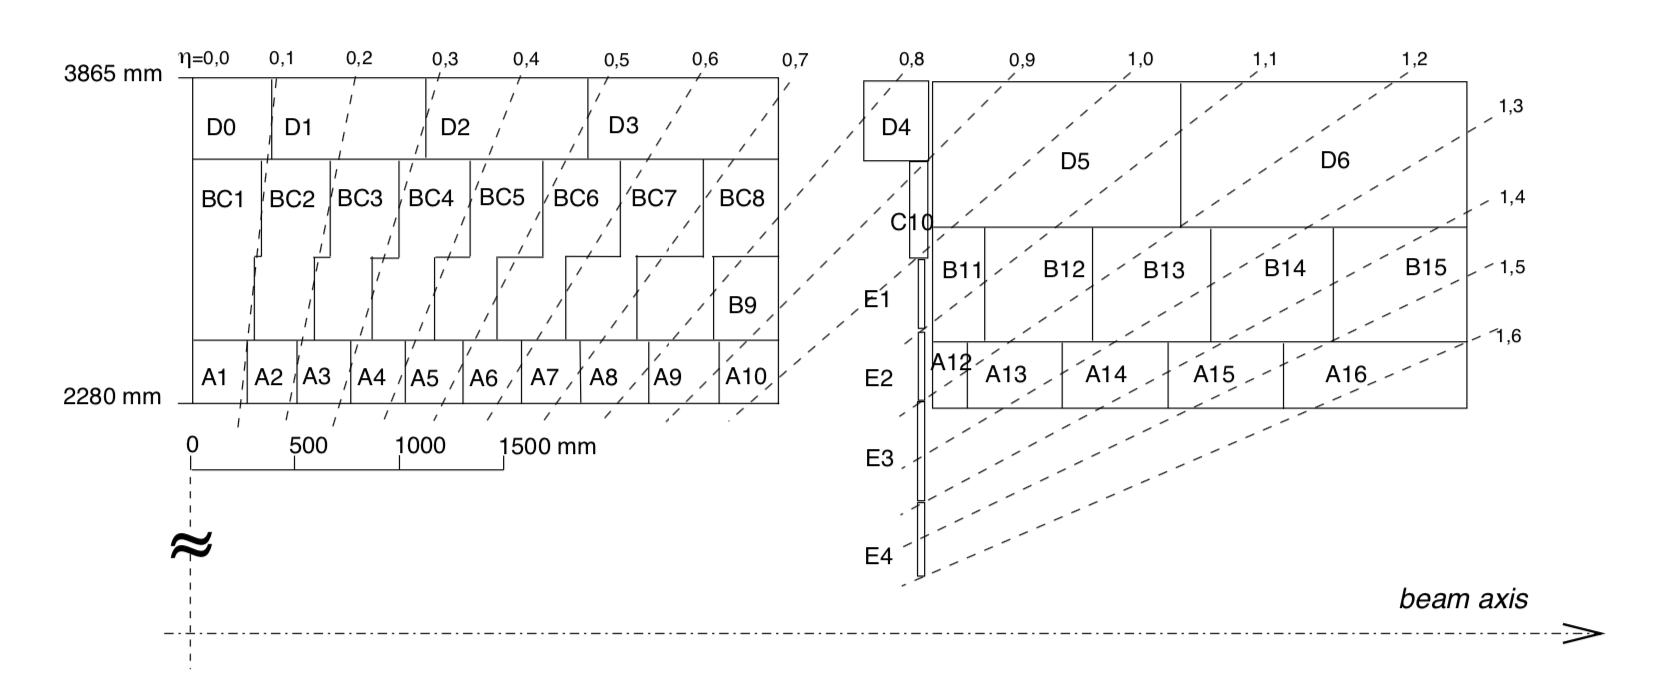
\includegraphics[width=\textwidth]{tile_cal_granularity}
\caption{Schematic of the central (left) and extended (right) tile calorimeter, showing the $\eta$- and depth-dependent segmentation.}
\label{fig:tile_cal_granularity}\cite{atlas-detector-2008}
\end{figure}

\subsubsection{Hadronic end-cap calorimeters}

The hadronic end-cap calorimeter (HEC) consists of two cylindrical wheels on each side of the barrel,
each of which is $2.03~m$ in radius.
Each of these wheels is made up of 32 modules.
The HEC wheels closest and farthest from the interaction point are called HEC1 and HEC2.
HEC1 modules have higher granularity and sample fraction than HEC2 modules.
A schematic of the HEC modules can be seen in figure~\ref{fig:hec_module}.

\begin{figure}[h]
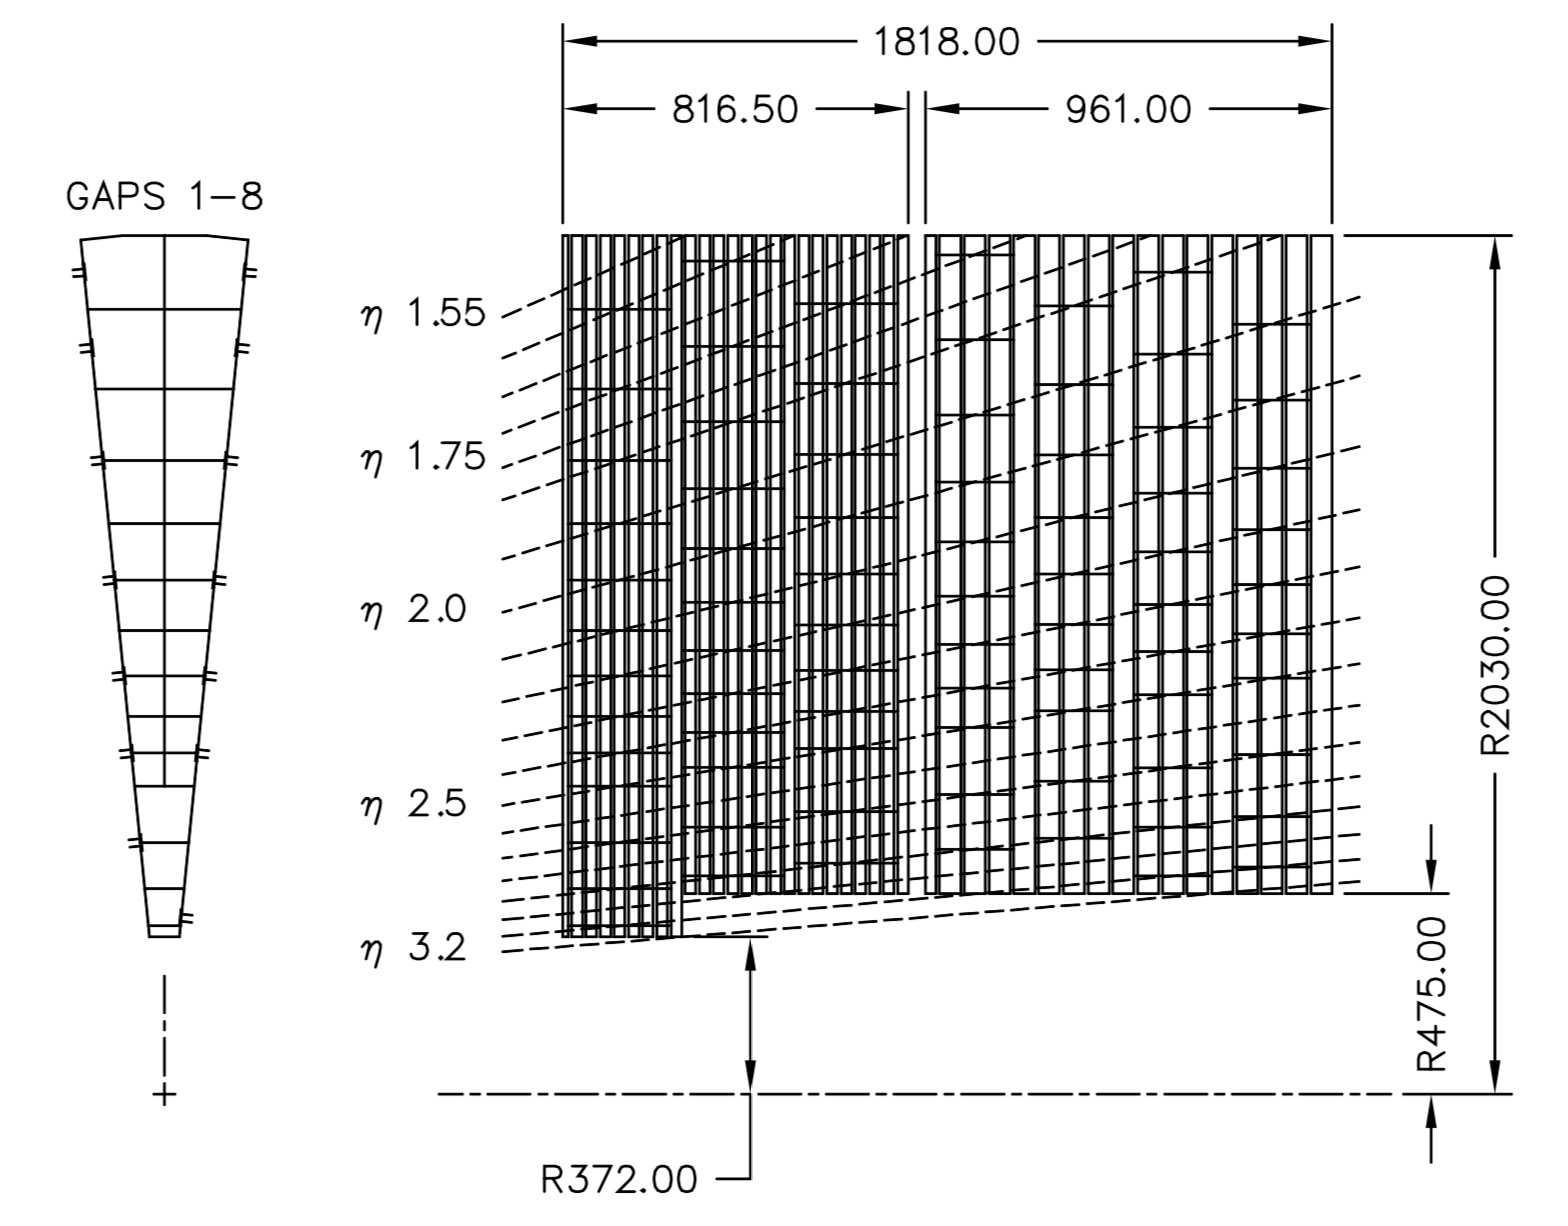
\includegraphics[width=\textwidth]{hec_module}
\caption{Schematic of hadronic end-cap calorimeter module}
\label{fig:hec_module}\cite{atlas-detector-2008}
\end{figure}

The HECs use LAr as the sampling material and copper as the absorber material.
The copper plates are separated by gaps of $8.5~mm$, with three electrodes in between.
This creates four drift zones between each copper plate.
Typical drift time across the drift zones is $430 ns$, at a potential difference of $1800 V$.\cite{atlas-detector-2008}

There are a total of 5632 readout cells.
In the region $|\eta| < 2.5$, the readout cell size is $\delta\phi \times \delta\eta = 0.1 \times 0.1$, and $\delta\phi \times \delta\eta = 0.2 \times 0.2$ elsewhere.

\subsection{Forward Calorimeters}\label{subsec:fcal}

Special forward calorimeters (FCal) were designed to cover the forward region, $3.1 < |\eta| < 4.9$.
This region experiences very high particle flux compared to the barrel or end-cap regions, so a different design was needed.
Each FCal consists of three modules.
The module closest to the interaction point (FCal1)is optimized for EM showers,
while the middle and outer modules (FCal2 and FCal3) are optimized for hadronic showers.
All three modules are $45~cm$ deep, and use LAr as the sampling material.

FCal1 uses copper as the absorber material, while FCal2 and FCal3 use tungsten as the primary absorber.
To further reduce punch-through into the muon system, a copper shield plug is placed behind FCal3.

The location of the FCal with respect to the end-cap calorimeters can be seen in figure~\ref{fig:fcal_layout}
The FCal, hadronic end-cap, and electromagnetic end-cap calorimeters are all contained in the same end-cap cryostat.

The overlapping design of the end-cap and forward calorimeters allows for hermetic coverage with minimal energy loss out to $|\eta| < 4.9$.

\begin{figure}[h]
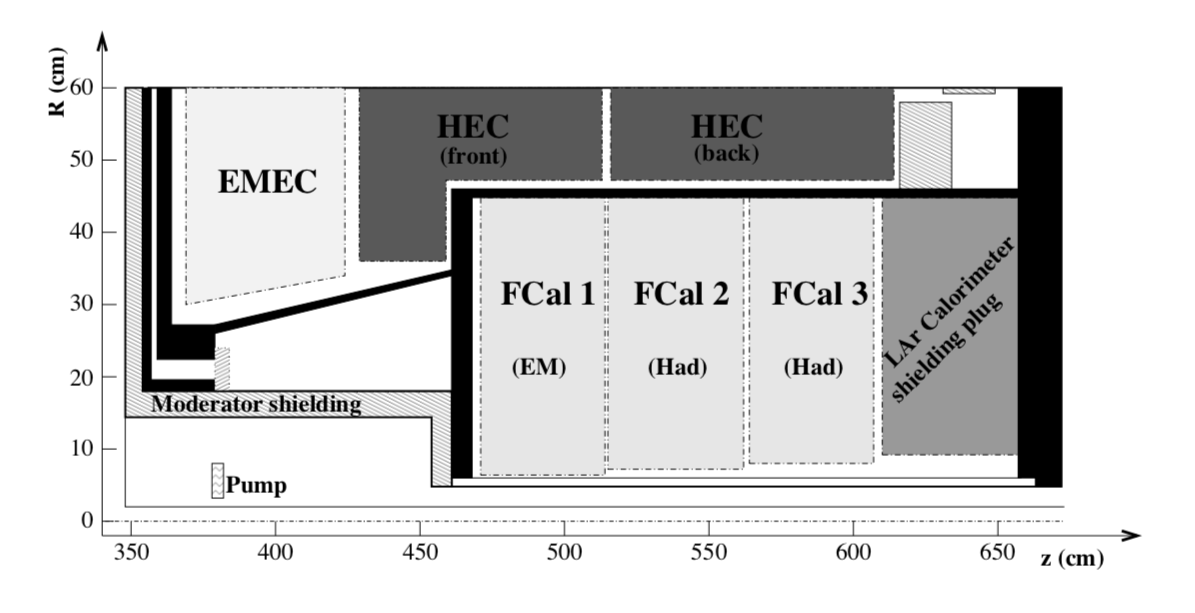
\includegraphics[width=\textwidth]{fcal_layout}
\caption{Schematic showing the layout of the forward calorimeters and end-cap calorimeters.}
\label{fig:fcal_layout}\cite{atlas-detector-2008}
\end{figure}

\subsubsection{Energy absorbtion}
In order to provide accurate energy measurements of photons, jets, and $E_{Tmiss}$,
it is necessary for the calorimeters to absorb as much shower energy as possible.
Any particles that don't get absorbed by the calorimeter are considered punch-through particles.
These punch-through particles add noise to the muon system, and so should be minimized.

For hadronic showers, the analog to a radiation length is called an interaction length, $\lambda$ .
The amount of energy absorbed by each part of the calorimeter, as measured in radiation lengths, can be seen in figure~\ref{fig:calo_material_budget}.

\begin{figure}[h]
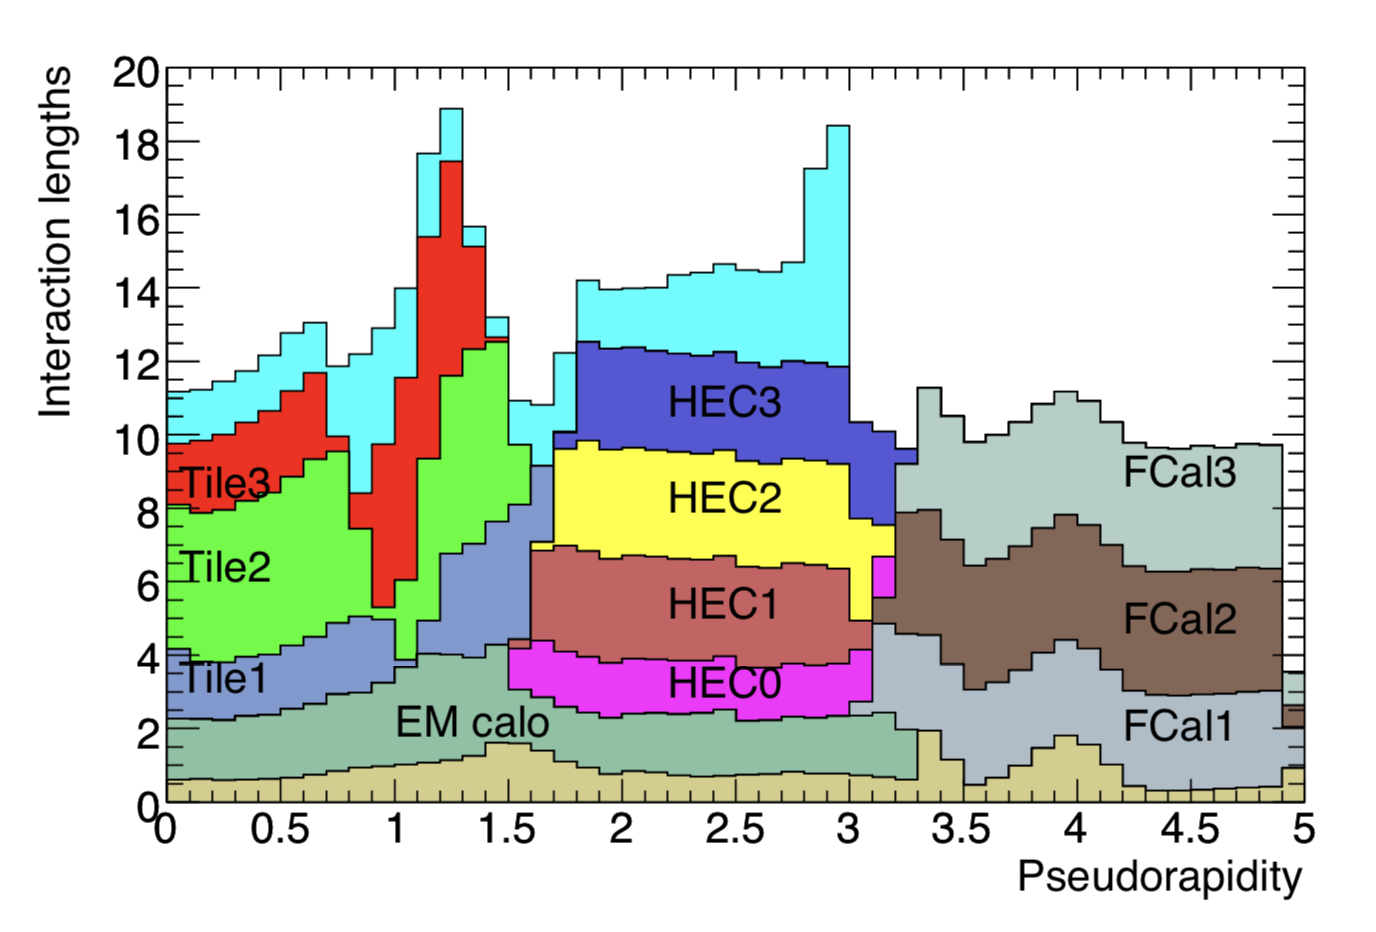
\includegraphics[width=\textwidth]{calo_material_budget}
\caption{Amount of material, in units of interaction length, versus pseudorapidity, including all material before the
EM calorimeter, the EM calorimeter, and the hadronic calorimeters. The light blue indicates the amount of material in front
of the muon spectrometer for $|\eta| < 3.0$}
\label{fig:calo_material_budget}\cite{atlas-detector-2008}
\end{figure}

\section{Muon Spectrometer}\label{sec:muon_spec}

The outermost ATLAS system is the muon spectrometer, used to measure the momenta of charged particles that exit the calorimeter systems.
Muons are not absorbed by the EM calorimeter because they undergo less bremsstrahlung than electrons due to their high mass.
They are also no absorbed by the hadronic calorimeter because they do not interact strongly.
As a result, muons are the most common particle to escape the calorimeter system.

The overall dimensions of the muon spectrometer, which define the demensions of ATLAS, are $44~m$ long by $22~m$ high.
The muon spectrometer consists of four subsystems.
The monitored drift tubes (MDTs) and cathode strip chambers (CSCs) are used for high-precision tracking,
while the resistive plate chambers (RDCs) and thin-gap chambers (TGCs) are used for triggering and bunch-crossing identification.
The location of each of the four muon subsystems can be seen in figure~\ref{fig:muon_spec_layout}

\begin{figure}[!htbp]
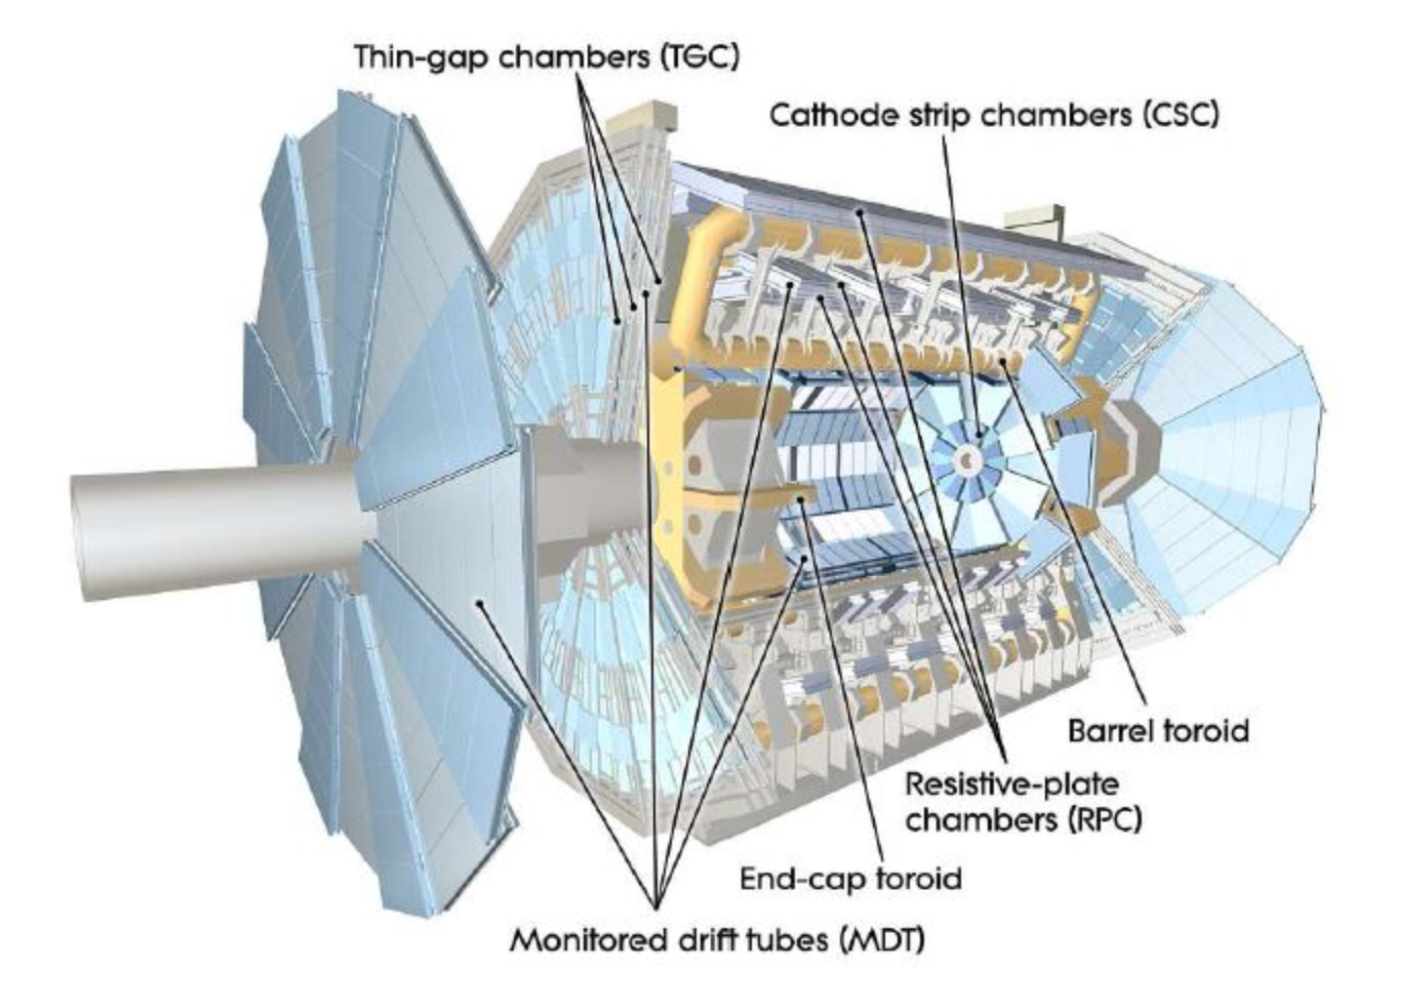
\includegraphics[width=\textwidth]{muon_spec_layout}
\caption{Layout of the muon spectrometer, indicating the location of barrel and end-cap toroids, along with the four subsystems.}
\label{fig:muon_spec_layout}\cite{atlas-detector-2008}
\end{figure}

As described in section~\ref{sec:magnet_systems}, the magnetic field in the muon system runs in a roughly circular direction around the beamline.
As a result, charged particles are bent in the $\eta$ direction in the muon spectrometer.

In the barrel region, covering $|\eta| < 1.0$ the muon system is laid out in three concentric cells,
located at $5~m$, $7.5~m$, and $10~m$ from the interaction point.
Full coverage is provided in this region, except for a small gap at $|\eta| = 0$, to allow for services to the solenoid,
calorimeters, and inner detector systems.
The size of the acceptance gap is $|\eta| < 0.04$ in the innermost layer, and $|\eta| < 0.08$ in the outer layers.
The end-cap consists of large wheels, located at $|z| \approx 7.4~m$, $10.8~m$, $14~m$, and $21.5~m$.
Figure~\ref{fig:muon_cross_section} shows a cross-section of the barrel region of the muon spectrometer in the $x-y$ plane,
and a cross-section of the barrel and end-cap regions in the $y-z$ plane.
The small acceptance gap at $\eta = 0$ can be seen.

\begin{figure}[!htbp]
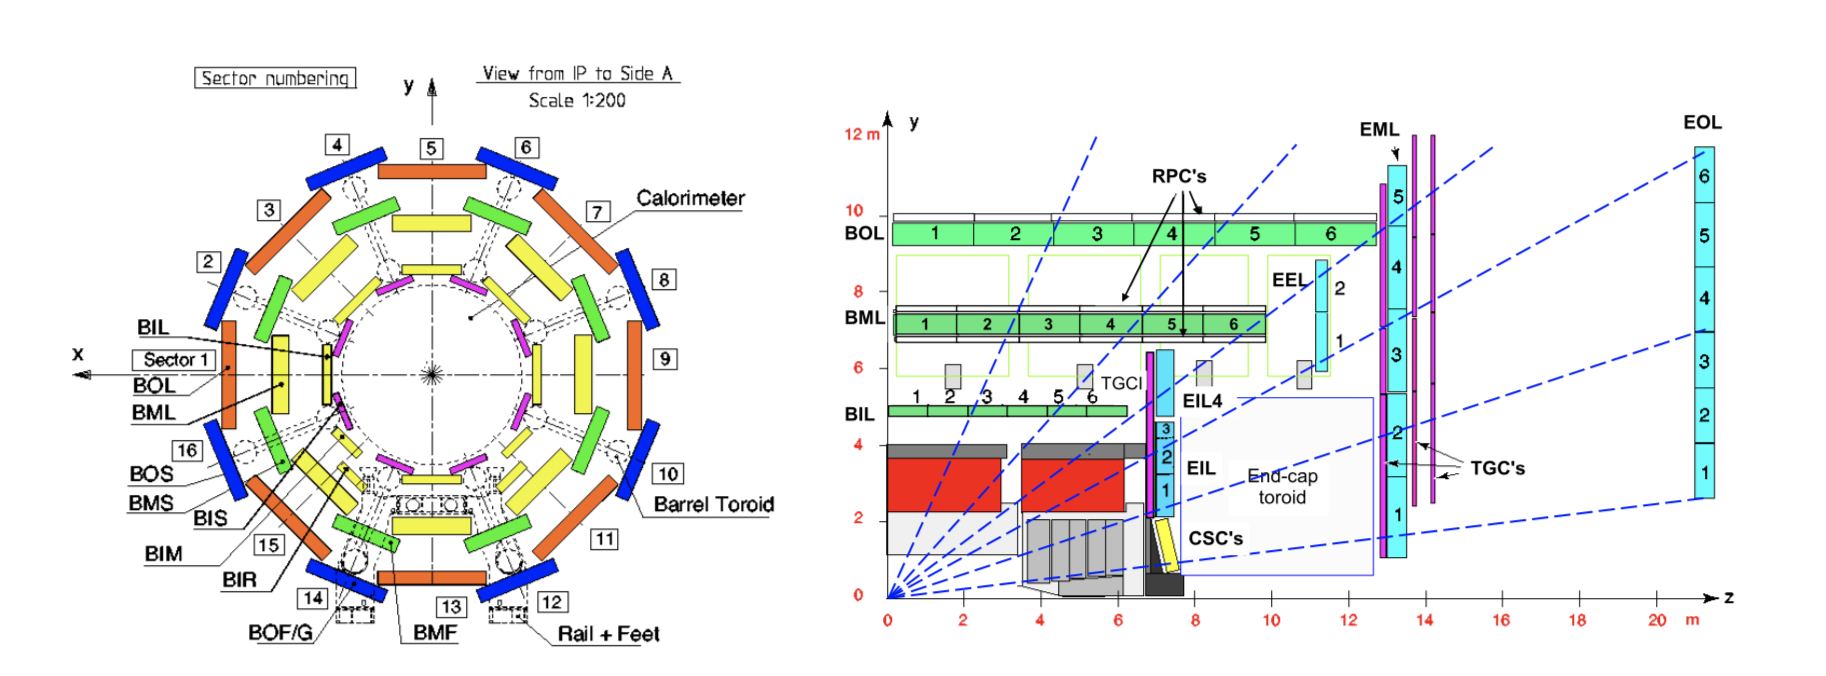
\includegraphics[width=\textwidth]{muon_cross_section}
\caption{Cross-sections in $x-y$ (left) and $y-z$ (right) of the muon spectrometer.}
\label{fig:muon_cross_section}\cite{muon-2003}
\end{figure}

The muon spectrometer provides high-precision momentum measurements out to $|\eta| < 2.7$,
and triggering on high-momentum muons out to $|\eta| < 2.4$.

The ATLAS design specification requires momentum resolution of $10\%$ for $1~TeV$ muons.
This resolution is achieved or exceeded for the range $10~GeV < p_T < 1~TeV$.
The contribution to $p_T$ resolution from various sources at different $p_T$ is shown in figure~\ref{fig:muon_resolution}.
The dominant contribution at low-$p_T$ is from energy loss fluctuations,
while at high-$p_T$ it's from wire resolution and autocalibration.\cite{muon-2003}

\begin{figure}[h]
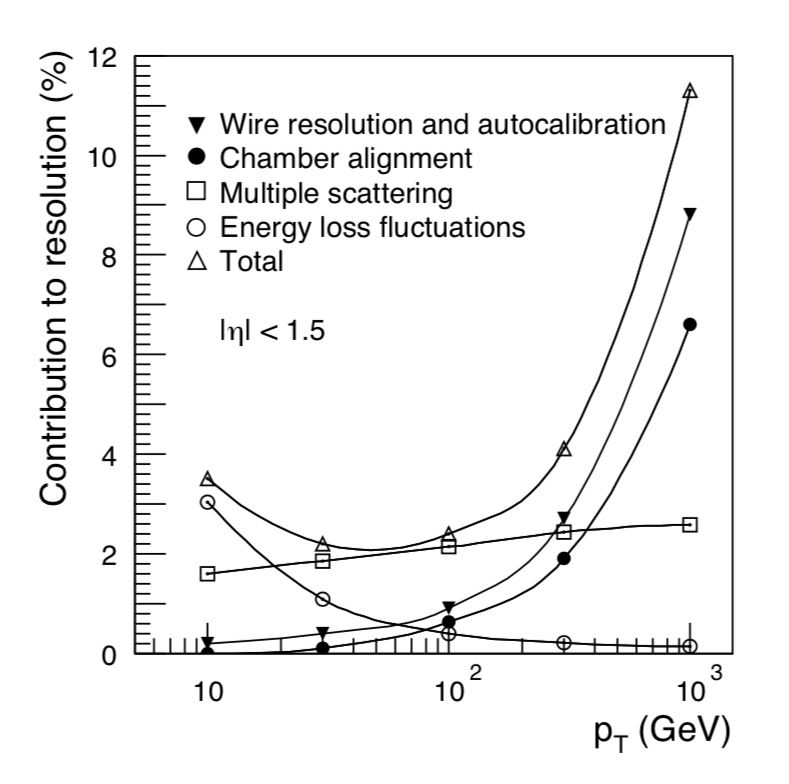
\includegraphics[width=\textwidth]{muon_pt_resolution}
\caption{The contribution to muon spectrometer $p_T$ resolution from various sources over a range of $p_T$}
\label{fig:muon_resolution}\cite{muon-2003}
\end{figure}

\subsubsection{Monitored drift tubes (MDTs)}
Most of the precision momentum measurements in the muon spectrometer are performed by MDTs.
The MDT subsystem covers the region $|\eta| < 2.7$, except for the innermost end-cap layer,
where they cover out to $|\eta| = 2.0$.
There are a total of 1174 MDT chambers, each made up of between 3 and 8 layers of drift tubes.
The aluminum tubes are $3~cm$ in diameter and range between $0.9~m$ and $6.2~m$ in length.
They are filled with a mixture of $80~\% \mathrm{Ar}$ and  $20~\% \mathrm{CO_2}$.
The MDTs provide a resolution of $80~\mu m$ per tube, and $35~\mu m$ per chamber.

In order to provide high-precision measurements, the locations of all chambers and their support structures are constantly monitored.
Temperature and magnetic field conditions are also monitored, in order to account for thermal expansion and changes to drift time.\cite{muon-2003}

The MDTs can be safely operated at a rate of up to $150~Hz/cm^2$.
In the forward region of the innermost end-cap, where the background rate is highest, CSCs are used in place of MDTs.

\subsubsection{Cathode strip chambers (CSCs)}

In the innermost end-cap layer, covering the region $2.0 > |\eta| > 2.7$,
the background rate is too high for safe operation of MDTs.
Instead, precision momentum measurements are performed using cathode strip chambers,
which can be safely operated at rates up to $1000~Hz/cm^2$\cite{atlas-detector-2008}.

The CSC chambers use the same gas mixture as MDT chambers.
Instead of drift tubes there are grids of anodes and cathodes, allowing for measurements of $\eta$ and $\phi$ based on
the charge induced in the wires.

There are a total of 32 CSC chambers, arranged into 4 disks of 8 chambers each.
Each chamber contains 4 CSC layers, resulting in 4 independent measurements of $\eta$ and $\phi$ for each track.
Cathodes are made of $17~mm$ copper strips, and anodes are gold-plated tungsten measuring $30~mm$ in diameter.
Sense-wire pitch is $2.54~mm$, but resolution is limited by readout pitch, which is $5.08~mm$.
This results in an $\eta$ resolution of $60~\mu m$, and a $\phi$ resolution of $5~mm$.\cite{muon-2003}
Since the magnetic fields bend muons in the $\eta$ plane, precice momentum measurements require far greater resolution in $\eta$.

\subsubsection{Resistive plate chambers (RPCs)}

Resistive plate chambers are used for the muon trigger in the barrel region $|\eta| < 1.05$.
In the middle station, there are two layers of RPCs, used for the low-$p_T$ threshold trigger.
This trigger threshold is $6-9~GeV$.
In the outer station, there is a single layer of RPCs, used for the high-$p_T$ threshold trigger,
with a threshold of $9-35~GeV$.

Each RPC consists of two rectangular detectors, called units.
Standard RPCs are paired with MDTs, and have the same dimensions.
A few additional smaller RPCs are included in areas where MDTs cannot be installed due to lack of space.

Each RPC provides two measurements of $\eta$ and $\phi$ for a charged particle passing through it.
A charged particle passing through all three layers therefore generates 6 $\eta-\phi$ measurements.
To reduce fake tracks, 3 out of 4 of the middle-station detectors and at least one outer layer station must register hits.

An RPC detector consists of two plastic insulating plates, separated by $2~mm$, with a gas occupying the internal space.
A voltage difference of $9.8~kV$ is applied across the plates.
Charged particles passing through the plates generate an avalanche of charge which can then be measured by metallic strips connected to the plates.
The insulator plates are made of phenolic-melaminic plastic laminate,
and the gas is a mixture of $\mathrm{C_2 H_2 F4}$, $\mathrm{Iso-C_4 H_{10}}$, and $\mathrm{SF_6}$
in the proportions $94.7\%$, $5\%$, $0.3\%$.\cite{atlas-detector-2008}

The RPCs provide a time resolution of $2~ns$.

\subsubsection{Thin-gap chambers (TGCs)}

In the forward region, $1.05 < |\eta| < 2.4$, muon triggering is provided by thin-gap chambers (TGCs).
TGCs also provide a $\phi$ measurement to complement the $\eta$ measurement provided by the MDTs.

In the MDT end-cap middle layer, there are seven layers of TGCs, and in the inner layer, there are 2 layers of TGCs.
Each TGC layer consists of two concentric rings..

Like the CSCs, the TGCs are multi-wire proportional chambers (MWPCs).
To reduce drift time so that an acceptable time resolution can be achieved, the drift distance must be kept small,
and the electric field kept high.
The wire-to-cathode distance is $1.4~mm$ in the TGCs, even closer than the wire-to-wire distance of $1.8~mm$.
The voltage is kept at $2.9~kV$.
A highly quenching gas mixture of $55\% \mathrm{CO_2}$ and $45\% \mathrm{n-C_5 H_{12}}$ is used in the TGCs.\cite{atlas-detector-2008}

The time resolution provided by the TGCs is $4~ns$.\cite{muon-2003}

\section{Trigger}\label{sec:trigger}

Because of the very high event rate at the LHC, and the large amount of data collected per event,
it is impossible to record every single event.
There are 40 million events per second, and each event generates $1.6~MB$ of raw data.
The ATLAS trigger system is designed to make very fast decisions about which events to record and which to ignore,
in order to reduce the event rate to approximately $1~kHz$.
The challenge of trigger design is to balance processing time against decision accuracy,
to make sure that events that could be useful for physics analysis are not lost.
The selection criteria used by each level of the trigger are known as the trigger menu.
A large number of possible trigger selection criteria are designed, in order to serve the broad range of physics analyses performed at ATLAS .

The ATLAS trigger system consists of a hardware based level 1 (L1) trigger, and a software-based high-level trigger (HLT).
The L1 trigger reduces the event rate from the original $40~MHz$ to approximately $100~kHz$.
The HLT further reduces the event rate to approximately $1~kHz$, which is the maximum rate of data transfer from the detector.
The flowchart of data through the trigger system can be seen in figure~\ref{fig:trigger_flowchart}

\begin{figure}[!htbp]
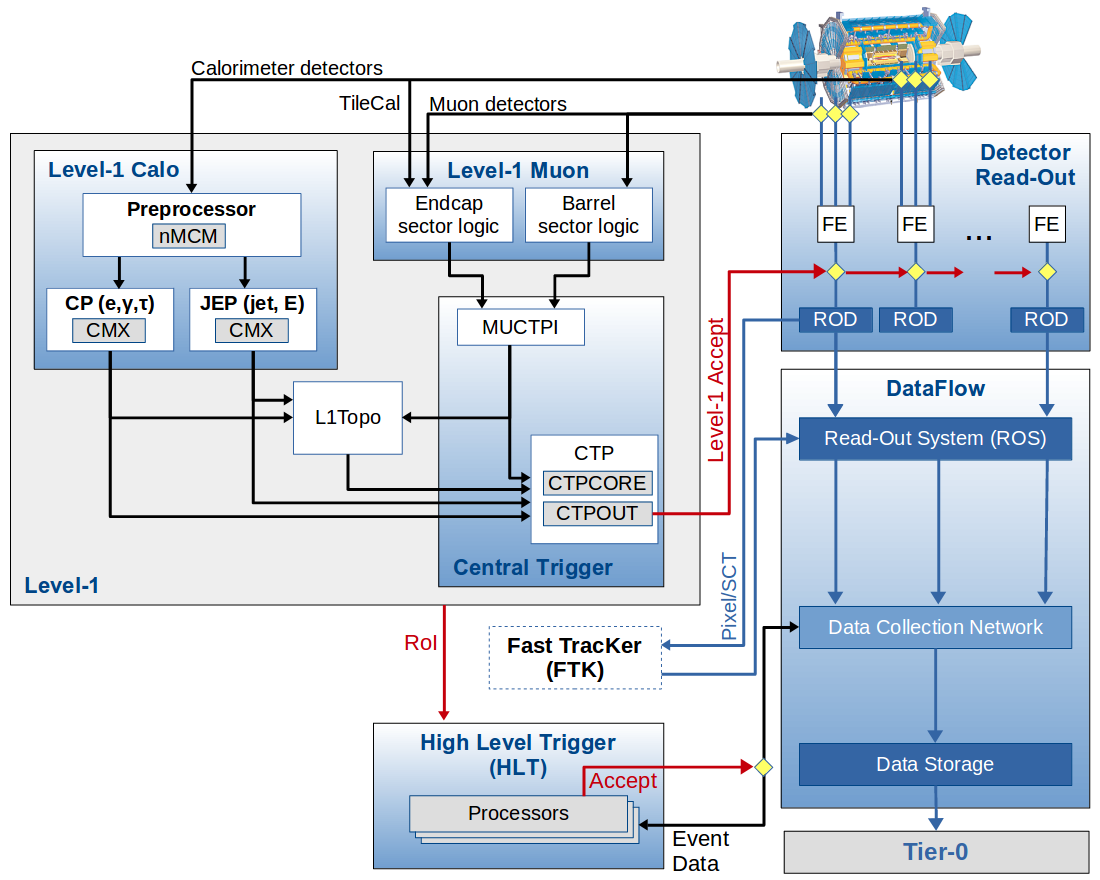
\includegraphics[width=\textwidth]{trigger_flowchart}
\caption{Flowchart outlining the level 1 and high-level trigger design and data acquisition system.}
\label{fig:trigger_flowchart}
\end{figure}

For every event, the L1 trigger system reads reduced-granularity measurements from both the hadronic and electromagnetic calorimeters.
Special calorimeter cells, called trigger towers, in each calorimeter were designed for this purpose.
The trigger towers have a granularity of $\delta \eta \times \delta \phi = 0.1 \times 0.1$.
The location of the trigger towers at the back of the electromagnetic calorimeter can be seen in figure~\ref{fig:em_calo}.
The L1 trigger also reads data from the RPCs and TGCs of the muon spectrometer system, as discussed in~\ref{sec:muon_spec}.
The calorimeter data will be used for photon, electron, tau, jet, and $E_{Tmiss}$ triggers, and the muon data will only be used for muon triggers.
Data from these two sources are fed into the central trigger processor (CTP),
which makes the decision about whether or not accept each event at level 1.

If an event is accepted at L1, full detector raw data for that event is read out and temporarily stored until the HLT decision is made.
Some amount of reconstruction is done at this time, including a high-speed,
reduced-accuracy version of the tracking algorithms, known as Fast TracKer (FTK).
Later, if an event is accepted by the HLT, the full tracking reconstruction algorithm will be applied.
The L1 system then sends region-of-interest information to the HLT .
Regions of interest are the subsections of the detector that the L1 trigger has identified as possibly containing interesting physics objects.
The full detector information and L1 region-of-interest data are combined by the HLT,
which then makes the final decision on whether or not to keep an event.
Only when an event passes both the L1 and HLT decision criteria will its be permanently stored.

The L1 trigger system desicision time is just $2.5~\mu m$, while the HLT makes decsisons on the order of seconds.